
%% bare_jrnl.tex
%% V1.4b
%% 2015/08/26
%% by Michael Shell
%% see http://www.michaelshell.org/
%% for current contact information.
%%
%% This is a skeleton file demonstrating the use of IEEEtran.cls
%% (requires IEEEtran.cls version 1.8b or later) with an IEEE
%% journal paper.
%%
%% Support sites:
%% http://www.michaelshell.org/tex/ieeetran/
%% http://www.ctan.org/pkg/ieeetran
%% and
%% http://www.ieee.org/

%%*************************************************************************
%% Legal Notice:
%% This code is offered as-is without any warranty either expressed or
%% implied; without even the implied warranty of MERCHANTABILITY or
%% FITNESS FOR A PARTICULAR PURPOSE! 
%% User assumes all risk.
%% In no event shall the IEEE or any contributor to this code be liable for
%% any damages or losses, including, but not limited to, incidental,
%% consequential, or any other damages, resulting from the use or misuse
%% of any information contained here.
%%
%% All comments are the opinions of their respective authors and are not
%% necessarily endorsed by the IEEE.
%%
%% This work is distributed under the LaTeX Project Public License (LPPL)
%% ( http://www.latex-project.org/ ) version 1.3, and may be freely used,
%% distributed and modified. A copy of the LPPL, version 1.3, is included
%% in the base LaTeX documentation of all distributions of LaTeX released
%% 2003/12/01 or later.
%% Retain all contribution notices and credits.
%% ** Modified files should be clearly indicated as such, including  **
%% ** renaming them and changing author support contact information. **
%%*************************************************************************


% *** Authors should verify (and, if needed, correct) their LaTeX system  ***
% *** with the testflow diagnostic prior to trusting their LaTeX platform ***
% *** with production work. The IEEE's font choices and paper sizes can   ***
% *** trigger bugs that do not appear when using other class files.       ***                          ***
% The testflow support page is at:
% http://www.michaelshell.org/tex/testflow/



\documentclass[journal]{IEEEtran}
%
% If IEEEtran.cls has not been installed into the LaTeX system files,
% manually specify the path to it like:
% \documentclass[journal]{../sty/IEEEtran}





% Some very useful LaTeX packages include:
% (uncomment the ones you want to load)


% *** MISC UTILITY PACKAGES ***
%
%\usepackage{ifpdf}
% Heiko Oberdiek's ifpdf.sty is very useful if you need conditional
% compilation based on whether the output is pdf or dvi.
% usage:
% \ifpdf
%   % pdf code
% \else
%   % dvi code
% \fi
% The latest version of ifpdf.sty can be obtained from:
% http://www.ctan.org/pkg/ifpdf
% Also, note that IEEEtran.cls V1.7 and later provides a builtin
% \ifCLASSINFOpdf conditional that works the same way.
% When switching from latex to pdflatex and vice-versa, the compiler may
% have to be run twice to clear warning/error messages.






% *** CITATION PACKAGES ***
%
\usepackage{cite}
% cite.sty was written by Donald Arseneau
% V1.6 and later of IEEEtran pre-defines the format of the cite.sty package
% \cite{} output to follow that of the IEEE. Loading the cite package will
% result in citation numbers being automatically sorted and properly
% "compressed/ranged". e.g., [1], [9], [2], [7], [5], [6] without using
% cite.sty will become [1], [2], [5]--[7], [9] using cite.sty. cite.sty's
% \cite will automatically add leading space, if needed. Use cite.sty's
% noadjust option (cite.sty V3.8 and later) if you want to turn this off
% such as if a citation ever needs to be enclosed in parenthesis.
% cite.sty is already installed on most LaTeX systems. Be sure and use
% version 5.0 (2009-03-20) and later if using hyperref.sty.
% The latest version can be obtained at:
% http://www.ctan.org/pkg/cite
% The documentation is contained in the cite.sty file itself.






% *** GRAPHICS RELATED PACKAGES ***
%
\ifCLASSINFOpdf
  \usepackage[pdftex]{graphicx}
  % declare the path(s) where your graphic files are
  % \graphicspath{{../pdf/}{../jpeg/}}
  % and their extensions so you won't have to specify these with
  % every instance of \includegraphics
  % \DeclareGraphicsExtensions{.pdf,.jpeg,.png}
\else
  % or other class option (dvipsone, dvipdf, if not using dvips). graphicx
  % will default to the driver specified in the system graphics.cfg if no
  % driver is specified.
  % \usepackage[dvips]{graphicx}
  % declare the path(s) where your graphic files are
  % \graphicspath{{../eps/}}
  % and their extensions so you won't have to specify these with
  % every instance of \includegraphics
  % \DeclareGraphicsExtensions{.eps}
\fi
% graphicx was written by David Carlisle and Sebastian Rahtz. It is
% required if you want graphics, photos, etc. graphicx.sty is already
% installed on most LaTeX systems. The latest version and documentation
% can be obtained at: 
% http://www.ctan.org/pkg/graphicx
% Another good source of documentation is "Using Imported Graphics in
% LaTeX2e" by Keith Reckdahl which can be found at:
% http://www.ctan.org/pkg/epslatex
%
% latex, and pdflatex in dvi mode, support graphics in encapsulated
% postscript (.eps) format. pdflatex in pdf mode supports graphics
% in .pdf, .jpeg, .png and .mps (metapost) formats. Users should ensure
% that all non-photo figures use a vector format (.eps, .pdf, .mps) and
% not a bitmapped formats (.jpeg, .png). The IEEE frowns on bitmapped formats
% which can result in "jaggedy"/blurry rendering of lines and letters as
% well as large increases in file sizes.
%
% You can find documentation about the pdfTeX application at:
% http://www.tug.org/applications/pdftex





% *** MATH PACKAGES ***
%
\usepackage{amsmath}
% A popular package from the American Mathematical Society that provides
% many useful and powerful commands for dealing with mathematics.
%
% Note that the amsmath package sets \interdisplaylinepenalty to 10000
% thus preventing page breaks from occurring within multiline equations. Use:
%\interdisplaylinepenalty=2500
% after loading amsmath to restore such page breaks as IEEEtran.cls normally
% does. amsmath.sty is already installed on most LaTeX systems. The latest
% version and documentation can be obtained at:
% http://www.ctan.org/pkg/amsmath





% *** SPECIALIZED LIST PACKAGES ***
%
%\usepackage{algorithmic}
% algorithmic.sty was written by Peter Williams and Rogerio Brito.
% This package provides an algorithmic environment fo describing algorithms.
% You can use the algorithmic environment in-text or within a figure
% environment to provide for a floating algorithm. Do NOT use the algorithm
% floating environment provided by algorithm.sty (by the same authors) or
% algorithm2e.sty (by Christophe Fiorio) as the IEEE does not use dedicated
% algorithm float types and packages that provide these will not provide
% correct IEEE style captions. The latest version and documentation of
% algorithmic.sty can be obtained at:
% http://www.ctan.org/pkg/algorithms
% Also of interest may be the (relatively newer and more customizable)
% algorithmicx.sty package by Szasz Janos:
% http://www.ctan.org/pkg/algorithmicx


\usepackage{listings}
\lstset{
	basicstyle=\ttfamily,
	showstringspaces=false,
	breaklines=true,
	frame=single,
	frameround=tttt,
}

% *** ALIGNMENT PACKAGES ***
%
%\usepackage{array}
% Frank Mittelbach's and David Carlisle's array.sty patches and improves
% the standard LaTeX2e array and tabular environments to provide better
% appearance and additional user controls. As the default LaTeX2e table
% generation code is lacking to the point of almost being broken with
% respect to the quality of the end results, all users are strongly
% advised to use an enhanced (at the very least that provided by array.sty)
% set of table tools. array.sty is already installed on most systems. The
% latest version and documentation can be obtained at:
% http://www.ctan.org/pkg/array


% IEEEtran contains the IEEEeqnarray family of commands that can be used to
% generate multiline equations as well as matrices, tables, etc., of high
% quality.




% *** SUBFIGURE PACKAGES ***
%\ifCLASSOPTIONcompsoc
%  \usepackage[caption=false,font=normalsize,labelfont=sf,textfont=sf]{subfig}
%\else
%  \usepackage[caption=false,font=footnotesize]{subfig}
%\fi
% subfig.sty, written by Steven Douglas Cochran, is the modern replacement
% for subfigure.sty, the latter of which is no longer maintained and is
% incompatible with some LaTeX packages including fixltx2e. However,
% subfig.sty requires and automatically loads Axel Sommerfeldt's caption.sty
% which will override IEEEtran.cls' handling of captions and this will result
% in non-IEEE style figure/table captions. To prevent this problem, be sure
% and invoke subfig.sty's "caption=false" package option (available since
% subfig.sty version 1.3, 2005/06/28) as this is will preserve IEEEtran.cls
% handling of captions.
% Note that the Computer Society format requires a larger sans serif font
% than the serif footnote size font used in traditional IEEE formatting
% and thus the need to invoke different subfig.sty package options depending
% on whether compsoc mode has been enabled.
%
% The latest version and documentation of subfig.sty can be obtained at:
% http://www.ctan.org/pkg/subfig




% *** FLOAT PACKAGES ***
%
%\usepackage{fixltx2e}
% fixltx2e, the successor to the earlier fix2col.sty, was written by
% Frank Mittelbach and David Carlisle. This package corrects a few problems
% in the LaTeX2e kernel, the most notable of which is that in current
% LaTeX2e releases, the ordering of single and double column floats is not
% guaranteed to be preserved. Thus, an unpatched LaTeX2e can allow a
% single column figure to be placed prior to an earlier double column
% figure.
% Be aware that LaTeX2e kernels dated 2015 and later have fixltx2e.sty's
% corrections already built into the system in which case a warning will
% be issued if an attempt is made to load fixltx2e.sty as it is no longer
% needed.
% The latest version and documentation can be found at:
% http://www.ctan.org/pkg/fixltx2e


%\usepackage{stfloats}
% stfloats.sty was written by Sigitas Tolusis. This package gives LaTeX2e
% the ability to do double column floats at the bottom of the page as well
% as the top. (e.g., "\begin{figure*}[!b]" is not normally possible in
% LaTeX2e). It also provides a command:
%\fnbelowfloat
% to enable the placement of footnotes below bottom floats (the standard
% LaTeX2e kernel puts them above bottom floats). This is an invasive package
% which rewrites many portions of the LaTeX2e float routines. It may not work
% with other packages that modify the LaTeX2e float routines. The latest
% version and documentation can be obtained at:
% http://www.ctan.org/pkg/stfloats
% Do not use the stfloats baselinefloat ability as the IEEE does not allow
% \baselineskip to stretch. Authors submitting work to the IEEE should note
% that the IEEE rarely uses double column equations and that authors should try
% to avoid such use. Do not be tempted to use the cuted.sty or midfloat.sty
% packages (also by Sigitas Tolusis) as the IEEE does not format its papers in
% such ways.
% Do not attempt to use stfloats with fixltx2e as they are incompatible.
% Instead, use Morten Hogholm'a dblfloatfix which combines the features
% of both fixltx2e and stfloats:
%
% \usepackage{dblfloatfix}
% The latest version can be found at:
% http://www.ctan.org/pkg/dblfloatfix




%\ifCLASSOPTIONcaptionsoff
%  \usepackage[nomarkers]{endfloat}
% \let\MYoriglatexcaption\caption
% \renewcommand{\caption}[2][\relax]{\MYoriglatexcaption[#2]{#2}}
%\fi
% endfloat.sty was written by James Darrell McCauley, Jeff Goldberg and 
% Axel Sommerfeldt. This package may be useful when used in conjunction with 
% IEEEtran.cls'  captionsoff option. Some IEEE journals/societies require that
% submissions have lists of figures/tables at the end of the paper and that
% figures/tables without any captions are placed on a page by themselves at
% the end of the document. If needed, the draftcls IEEEtran class option or
% \CLASSINPUTbaselinestretch interface can be used to increase the line
% spacing as well. Be sure and use the nomarkers option of endfloat to
% prevent endfloat from "marking" where the figures would have been placed
% in the text. The two hack lines of code above are a slight modification of
% that suggested by in the endfloat docs (section 8.4.1) to ensure that
% the full captions always appear in the list of figures/tables - even if
% the user used the short optional argument of \caption[]{}.
% IEEE papers do not typically make use of \caption[]'s optional argument,
% so this should not be an issue. A similar trick can be used to disable
% captions of packages such as subfig.sty that lack options to turn off
% the subcaptions:
% For subfig.sty:
% \let\MYorigsubfloat\subfloat
% \renewcommand{\subfloat}[2][\relax]{\MYorigsubfloat[]{#2}}
% However, the above trick will not work if both optional arguments of
% the \subfloat command are used. Furthermore, there needs to be a
% description of each subfigure *somewhere* and endfloat does not add
% subfigure captions to its list of figures. Thus, the best approach is to
% avoid the use of subfigure captions (many IEEE journals avoid them anyway)
% and instead reference/explain all the subfigures within the main caption.
% The latest version of endfloat.sty and its documentation can obtained at:
% http://www.ctan.org/pkg/endfloat
%
% The IEEEtran \ifCLASSOPTIONcaptionsoff conditional can also be used
% later in the document, say, to conditionally put the References on a 
% page by themselves.




% *** PDF, URL AND HYPERLINK PACKAGES ***
%
\usepackage{url}
% url.sty was written by Donald Arseneau. It provides better support for
% handling and breaking URLs. url.sty is already installed on most LaTeX
% systems. The latest version and documentation can be obtained at:
% http://www.ctan.org/pkg/url
% Basically, \url{my_url_here}.

\usepackage[hidelinks]{hyperref}


% *** Do not adjust lengths that control margins, column widths, etc. ***
% *** Do not use packages that alter fonts (such as pslatex).         ***
% There should be no need to do such things with IEEEtran.cls V1.6 and later.
% (Unless specifically asked to do so by the journal or conference you plan
% to submit to, of course. )


% correct bad hyphenation here
\hyphenation{op-tical net-works semi-conduc-tor}

%\addbibresource{Bibliography.bib}


\begin{document}
%
% paper title
% Titles are generally capitalized except for words such as a, an, and, as,
% at, but, by, for, in, nor, of, on, or, the, to and up, which are usually
% not capitalized unless they are the first or last word of the title.
% Linebreaks \\ can be used within to get better formatting as desired.
% Do not put math or special symbols in the title.
\title{Integration of Idemix in IoT environments}
%
%
% author names and IEEE memberships
% note positions of commas and nonbreaking spaces ( ~ ) LaTeX will not break
% a structure at a ~ so this keeps an author's name from being broken across
% two lines.
% use \thanks{} to gain access to the first footnote area
% a separate \thanks must be used for each paragraph as LaTeX2e's \thanks
% was not built to handle multiple paragraphs
%

%\author{Jose Luis Canovas Sanchez, Antonio Skarmeta Gomez, Jorge Benal Bernabe}% <-this % stops a space


\author{\IEEEauthorblockN{Jose Luis Canovas Sanchez, Jorge Bernal Bernabe, Antonio F. Skarmeta}\\
	\IEEEauthorblockA{Department of Information and Communications Engineering\\
		Computer Science Faculty, 
		University of Murcia, Spain\\
		\{joseluiscanovas, jorgebernal, skarmeta\}@um.es\\
	}
}%



%\thanks{M. Shell was with the Department
%of Electrical and Computer Engineering, Georgia Institute of Technology, Atlanta,
%GA, 30332 USA e-mail: (see http://www.michaelshell.org/contact.html).}% <-this % stops a space
%\thanks{J. Doe and J. Doe are with Anonymous University.}% <-this % stops a space
%\thanks{Manuscript received April 19, 2005; revised August 26, 2015.}}

% note the % following the last \IEEEmembership and also \thanks - 
% these prevent an unwanted space from occurring between the last author name
% and the end of the author line. i.e., if you had this:
% 
% \author{....lastname \thanks{...} \thanks{...} }
%                     ^------------^------------^----Do not want these spaces!
%
% a space would be appended to the last name and could cause every name on that
% line to be shifted left slightly. This is one of those "LaTeX things". For
% instance, "\textbf{A} \textbf{B}" will typeset as "A B" not "AB". To get
% "AB" then you have to do: "\textbf{A}\textbf{B}"
% \thanks is no different in this regard, so shield the last } of each \thanks
% that ends a line with a % and do not let a space in before the next \thanks.
% Spaces after \IEEEmembership other than the last one are OK (and needed) as
% you are supposed to have spaces between the names. For what it is worth,
% this is a minor point as most people would not even notice if the said evil
% space somehow managed to creep in.



% The paper headers
%\markboth{Journal of \LaTeX\ Class Files,~Vol.~14, No.~8, August~2015}%
%{Shell \MakeLowercase{\textit{et al.}}: Bare Demo of IEEEtran.cls for IEEE Journals}
% The only time the second header will appear is for the odd numbered pages
% after the title page when using the twoside option.
% 
% *** Note that you probably will NOT want to include the author's ***
% *** name in the headers of peer review papers.                   ***
% You can use \ifCLASSOPTIONpeerreview for conditional compilation here if
% you desire.




% If you want to put a publisher's ID mark on the page you can do it like
% this:
%\IEEEpubid{0000--0000/00\$00.00~\copyright~2015 IEEE}
% Remember, if you use this you must call \IEEEpubidadjcol in the second
% column for its text to clear the IEEEpubid mark.



% use for special paper notices
%\IEEEspecialpapernotice{(Invited Paper)}




% make the title area
\maketitle

% As a general rule, do not put math, special symbols or citations
% in the abstract or keywords.
\begin{abstract}
In this paper we design a solution to integrate IBM's Identity Mixer into the IoT ecosystem, integrating its privacy-preserving capabilities thanks to the use of Zero-Knowledge Proof cryptography. To validate our design, we implemented a functional Proof of Concept written in C for IoT devices. The applications of such solution promise to improve both the security and privacy of IoT, which in recent years have proved to be compromised.
\end{abstract}

% Note that keywords are not normally used for peerreview papers.
%\begin{IEEEkeywords}
%IEEE, IEEEtran, journal, \LaTeX, paper, template.
%\end{IEEEkeywords}






% For peer review papers, you can put extra information on the cover
% page as needed:
% \ifCLASSOPTIONpeerreview
% \begin{center} \bfseries EDICS Category: 3-BBND \end{center}
% \fi
%
% For peerreview papers, this IEEEtran command inserts a page break and
% creates the second title. It will be ignored for other modes.
\IEEEpeerreviewmaketitle



\section{Introduction}

The IoT is a term with a wide range of interpretations \cite{Atzori20102787}, breafly, we can think of it as billions of devices, mainly resource constrained, that are interconnected between them, and the Internet, in order to achieve a goal.

Many of this objectives require the use of a great amount of data, and thanks to organizations like WikiLeaks, people are aware of the implications of their data on the Internet, demanding more security and privacy for it. This includes not only the data shared with others, where one must trust they will keep it safe, but it's also the data collected about us and that we don't have direct control over it.

In traditional M2M (Machine to Machine) environments the issues about security and privacy have already been treated deeply, but in the IoT world, due to it's recent and fast growth, lacks of those tools to solve autonomously these problems.

With the proliferation of IoT devices gathering as much information as they can with their sensors, the amount of data stored about anyone can be immense. And IoT has proved to not address neither security nor privacy, with recent events like the Mirai botnet DDoS attack on October 2016, considered the biggest DDoS in history \cite{jeyanthi:2017}, or the multiple vulnerabilities affecting house devices, like baby monitors \cite{rapid7babycam}.

To address this problem of privacy in the Internet, a recent approach is the concept of \textit{strong anonymity}, that conceals our personal details while letting us continue to operate online as a clearly defined individuals \cite{stronganonymity}. To achieve it, we must address a way to perform authentication and authorization in the most privacy-friendly approach. Attribute-based credentials and \textit{selective disclosure} allow to control what information we reveal, under a trusted environment.

Intuitively, an attribute-based credential can be thought of as a digital signature by the Issuer on a list of attribute-value pairs, e.g. the list \texttt{(fname=Alice, lname=Anderson, bdate=1977-05-10, nation=DE)} \cite{introCredIBM}.
The most straightforward way for the User to convince a Verifier of her list of attributes would be to simply transmit her credential to the Verifier.
With anonymous credentials, the User never transmits the credential itself, but rather uses it to convince the Verifier that her attributes satisfy certain properties – without leaking anything about the credential other than the shown properties. This has the obvious advantage that the Verifier can no longer reuse the credential to impersonate \texttt{Alice}. Another advantage is that anonymous credentials allow the User to reveal a selected subset of her attributes.
Stronger even, apart from showing the exact value of an attribute, the User can even convince the
Verifier that some complex predicate over the attributes holds, e.g. that her birth date was more than 18 years ago, without revealing the real date.

With usual symmetric and asymmetric cryptography it seems rather impossible to create such credentials, without an explosion of signatures over every possible combination. For this reason, current solutions rely on  Zero-Knowledge Proofs (ZKP), cryptographic methods that allow to proof knowledge of some data without disclosing it.

To understand how ZKPs work, in 1990 Guillou, Quisquater and Berson published in \textit{How to Explain Zero-Knowledge Protocols to Your Children} \cite{ZKPcave:story} a story about how Ali Baba proved that he knew the magic words to open the cave, but without revealing those words to anyone.

Based on ZKP properties, IBM has developed the Identity Mixer\footnote{Identity Mixer - \url{https://www.research.ibm.com/labs/zurich/idemix/}}, Idemix for short, protocol suite for privacy-preserving authentication and transfer of certified attributes. It allows user authentication without divulging any personal data. Users have a personal certificate with multiple attributes, but they can choose how many to disclose, or only give a proof of them, like being older than 18 years-old, living in a country without revealing the city, etc. Thus, no personal data is collected that needs to be protected, managed, and treated.

\begin{center}
	\textit{``If your personal data is never collected, it cannot be stolen.''}
\end{center}

%%%
So far, Idemix or privacy-ABCs have been successfully applied to deal with traditional Internet scenarios, in which users can authenticate and prove their attributes against Service provider. However, due to the reduced computational capabilities of certain IoT devices, it has not been yet considered for IoT scenarios. As we study in the state of the art chapter, current implementations are based on Java, which requires high computational and memory resources to be executed, and to the best of our knowledge, this is the first proposal that tries to apply an IoT solution for privacy-preserving authentication and authorization, based on Anonymous credential Systems, like Idemix.
%%5


As part of IBM's academic grant for \textit{Privacy Preserving Identity Management applied to IoT}, the goal of this project is to integrate Idemix with the IoT. It will be done using ABC4Trust's P2ABCE, a framework that defines a common architecture, policy language and data artifacts for an attribute based ecosystem, cryptographically based on either IBM's Idemix or Microsoft's U-Prove \footnote{P2ABCEngine \url{https://github.com/p2abcengine/p2abcengine}}. This gives us a standardized language to exchange Idemix's messages between IoT devices and any other P2ABCE actor.

Once the IoT devices can execute Idemix, the new step is to take advantage of it in other deployments. In a smart building, different privacy policies could protect sensitive data, like how many people there are, and their identities, where a thermostat would only need to know if the amount of people is between some boundaries, but in case of emergency, the police department could request all the information available. We think that the first approach to achieve these ideas is first to integrate Idemix in known IoT identity systems, like FIWARE project. 

\hfil


This document is structured as follows: In \autoref{ch:stateoftheart} we show a state of the art analysis through the history of Idemix and related works, analysing what is of the most interest for the IoT perspective; in \autoref{ch:design} we describe the formal design of the IoT and Idemix solution, and describe the PoC implementation developed; after an implementation, it is a must to validate it, as showed during the performance tests in \autoref{ch:validation}; finally, our conclusions and lines for future work are described in \autoref{ch:conclusions}.



\section{State of the art}\label{ch:stateoftheart}

In this project we will study Identity Mixer as an Attribute-Based Credentials (ABC) solution for privacy-preserving scenarios, but there exist other solutions competing to give the best performance and capabilities as possible. The two most notable alternatives to Idemix are Microsoft's U-Prove and Persiano's ABC systems.


%%%%%%%%%%%%%%%%%%%%%%%%


Persiano and Visconti presented a non-transferable anonymous
credential system that is multi-show and for which it is possible to prove
properties (encoded by a linear Boolean formula) of the credentials \cite{book:185217}. Unfortunately, their proof system is not efficient since the step in which a user proves
possession of credentials (that needs a number of modular exponentiations that
is linear in the number of credentials) must be repeated times (where is the
security parameter) in order to obtain a satisfying soundness.

%%%%%%%%%%%%%%%%%%%%%%%%%


%%%%%%%%%


Stefan Brands provided the first integral description of the U-Prove
technology in his thesis \cite{uprove} in 2000, after which he founded the company Credentica
in 2002 to implement and sell this technology. Microsoft acquired Credentica
in 2008 and published the U-Prove protocol specification \cite{uprove2} in 2010
under the Open Specification Promise4 together with open source reference software
development kits (SDKs) in C\# and Java.
The U-Prove technology is centered around a so-called U-Prove token. This
token serves as a pseudonym for the prover. It contains a number of attributes
which can be selectively disclosed to a verifier. Hence the prover decides which
attributes to show and which to withhold. Finally there is the token’s public-key, which aggregates all information in the token, and a signature from the issuer
over this public-key to ensure the authenticity \cite{book:947508}.

%%%%%%%%%%%


\hfil

Jan Camenisch, Markus Stadler and Anna Lysyanskaya studied in \cite{Camenisch:GroupSig}, \cite{Camenisch:AnonCred} and \cite{camenisch2002signature} the cryptographic bases for signature schemes and anonymous credentials, that later became IBM's Identity Mixer protocol specification \cite{idemixSpec}.


Luuk Danes in 2007 studied theoretically how Idemix's User role could be implemented using  
smart cards \cite{luuk}, identifying what data and operations should be kept inside the device to perform different levels of security. The User role was divided between the smart card, holding secret keys, and the Idemix terminal, that commanded operations inside the smart card, or read the keys in it to perform the instructions itself. The studied sets were:
\begin{itemize}
	\item The smart card gives all information to the terminal.
	\item The smart card only keeps the master key secret.
	\item The smart card only gives the pseudonym with the verifier to the terminal.
	\item The smart card keeps everything secret.
\end{itemize}
%%%%

Later, in 2008 Víctor Sucasas also studied an anonymous credential system with smart card support \cite{sucasas}, equivalent to a basic version of Idemix, using a simulator to test the PoC and pointing out some crucial implementation details for performance. The researching tendency starts to show that smart cards are the best solution to hold safely the User's credentials.

In 2009, some Java smart card PoC for Idemix were developed in \cite{javaIdemix1} and \cite{javaIdemix2}, but they weren't optimal and didn't include some Idemix's functionalities, like selective disclosure.

Later, in 2013, Vullers and Alpar, implemented an efficient smart card for Idemix \cite{vullers2013efficient}, aiming to integrate it in the IRMA\footnote{The IRMA project has been recently included in the Privacy by Design Foundation: \url{https://privacybydesign.foundation/}} project, and comparing the performance with U-Prove's smart cards. This new implementation was written in C, under the MULTOS platform for smart cards, and describes many decisions made during the development to improve the performance on such constrained devices. The terminal application was written in Java and used an extension of the Idemix cryptographic library to take care of the smart card specifics.


Extending the concept of smart cards, physical or logical, as holders of the credentials, the ABC4Trust's project, P2ABCE\footnote{\url{https://github.com/p2abcengine/p2abcengine}}, was created as a unified ABC system for different cryptographic engines, currently supporting U-Prove and Idemix. The Idemix library was updated to support P2ABCE and the last version is interoperable with U-Prove. Therefore, the smart card specification from the P2ABCE project could be considered the official version to work with.


% Uso de P2ABCE en VANETs
Related to the IoT, the P2ABCE project has been used to test in a VANET\footnote{Vehicular Ad-Hoc Network} scenario how an OBU (On Board Unit), with constrained hardware, could act as a User in an P2ABC system \cite{vanet}. However, after the theoretical analysis, the paper only simulates a computer with similar performance as an OBU, without adapting the existing Java implementation of P2ABCE to a real VANET system. In our project, we can consider ourselves as part of their \textit{future work}, because our PoC will run on hardware actually used in VANET systems, and has been implemented in C instead of Java, which is more realistic and efficient for its deployment in an OBU.

%%%%%%%%%%%%%%







\section{Design and implementation}\label{ch:design}


We now proceed describe the design of our proposal to integrate IoT constrained devices as part of the privacy preserving system P2ABCE. The ultimate goal is to enable constrained IoT devices to play the Idemix User role, interacting autonomously in order to authenticate and demonstrate their credential attributes in a privacy-preserving fashion.

\subsection{Design}

In this section we will define how an IoT device may be integrated in the P2ABCE architecture, being totally compatible with any other system using P2ABCE, addressing the power and memory constrains many IoT devices face.

We decided to use P2ABCE with the Idemix as its Engine, because it is officially supported by the Idemix Library, it has the most up-to-date implementation, as we saw in the state of the art, and adds capabilities to Idemix like the Presentation Policies, or interoperability with U-Prove, not available without the P2ABCE project.

Our main goal is to make an IoT device capable to act as a User or Verifier in the P2ABCE architecture. For this, the device should be able to \textbf{communicate} with the Verifier or Prover with which it is interacting, manage the P2ABCE complex \textbf{XML schemas} transmitted, and perform the \textbf{cryptographic operations} required.

The communication between actors depends on each IoT scenario, it can be achieved with many existing standard solutions, e.g. an IP network, a Bluetooth M2M connection, RF communication, etc.

Our real concerns are, on one side, parsing the XML data, based on the P2ABCE's XML schema, that specifies the data artifacts created and exchanged during the issuance, presentation, revocation and inspection of pABCs; and on the other side, the cryptographic operations, that involve the use of secret keys, stored privately in the IoT device.

After the analysis done in the previous sections to the P2ABCE architecture, emphasizing that the logic of smart cards gathers the cryptographic operations independently from how the data is exchanged between P2ABCE actors. 

Using the \textit{computation offloading} technique to our scenario, our design consists on implementing the smart card logic inside the IoT device, keeping secure our master key and credentials, and for the rest of the P2ABCE system, if the device can not run the complete Engine, it may delegate to a server running it, indicating how to send APDU Commands to the \textit{IoT smart card}.

Even in the case we were to implement all P2ABCE inside an IoT device, we would have to implement the support for software smart cards, to keep the secret inside the IoT device. Therefore, we can begin implementing the smart card logic inside the IoT device, and later, if the device resources admit it, other components of the P2ABCE project.


\hfil

Computation offloading is not new to IoT deployments. For example, IPv6 involves managing 128 bits per address and other headers, and many IoT scenes only need to communicate inside a private network, making only the last 64 bits in an address relevant. To reduce that overhead, instead of IPv6 they use 6LoWPAN to compress packets and use smaller address sizes. To communicate a 6LoWPAN with the Internet or other networks, the IoT devices delegate the networking workload on a proxy that can manage the 6LoWPAN and IPv6 stacks. In the scope of consumer devices, smart bands or watches can install applications, bit many of them delegate on the user's phone to accomplish their task.

Therefore, the IoT device now has a \textbf{duality} in its functions, because it is the User that starts any interaction with other actors, and it's also the smart card that a P2ABCE server must ask for cryptographic operations. It can also be seen as a \textbf{double delegation}. The IoT device delegates on the external P2ABCE server to manage the protocol, and the P2ABCE server delegates on the IoT, acting now as a smart card, for the cryptography.

\subsubsection{System architecture}



\begin{figure}[bth]
	\begin{center}
		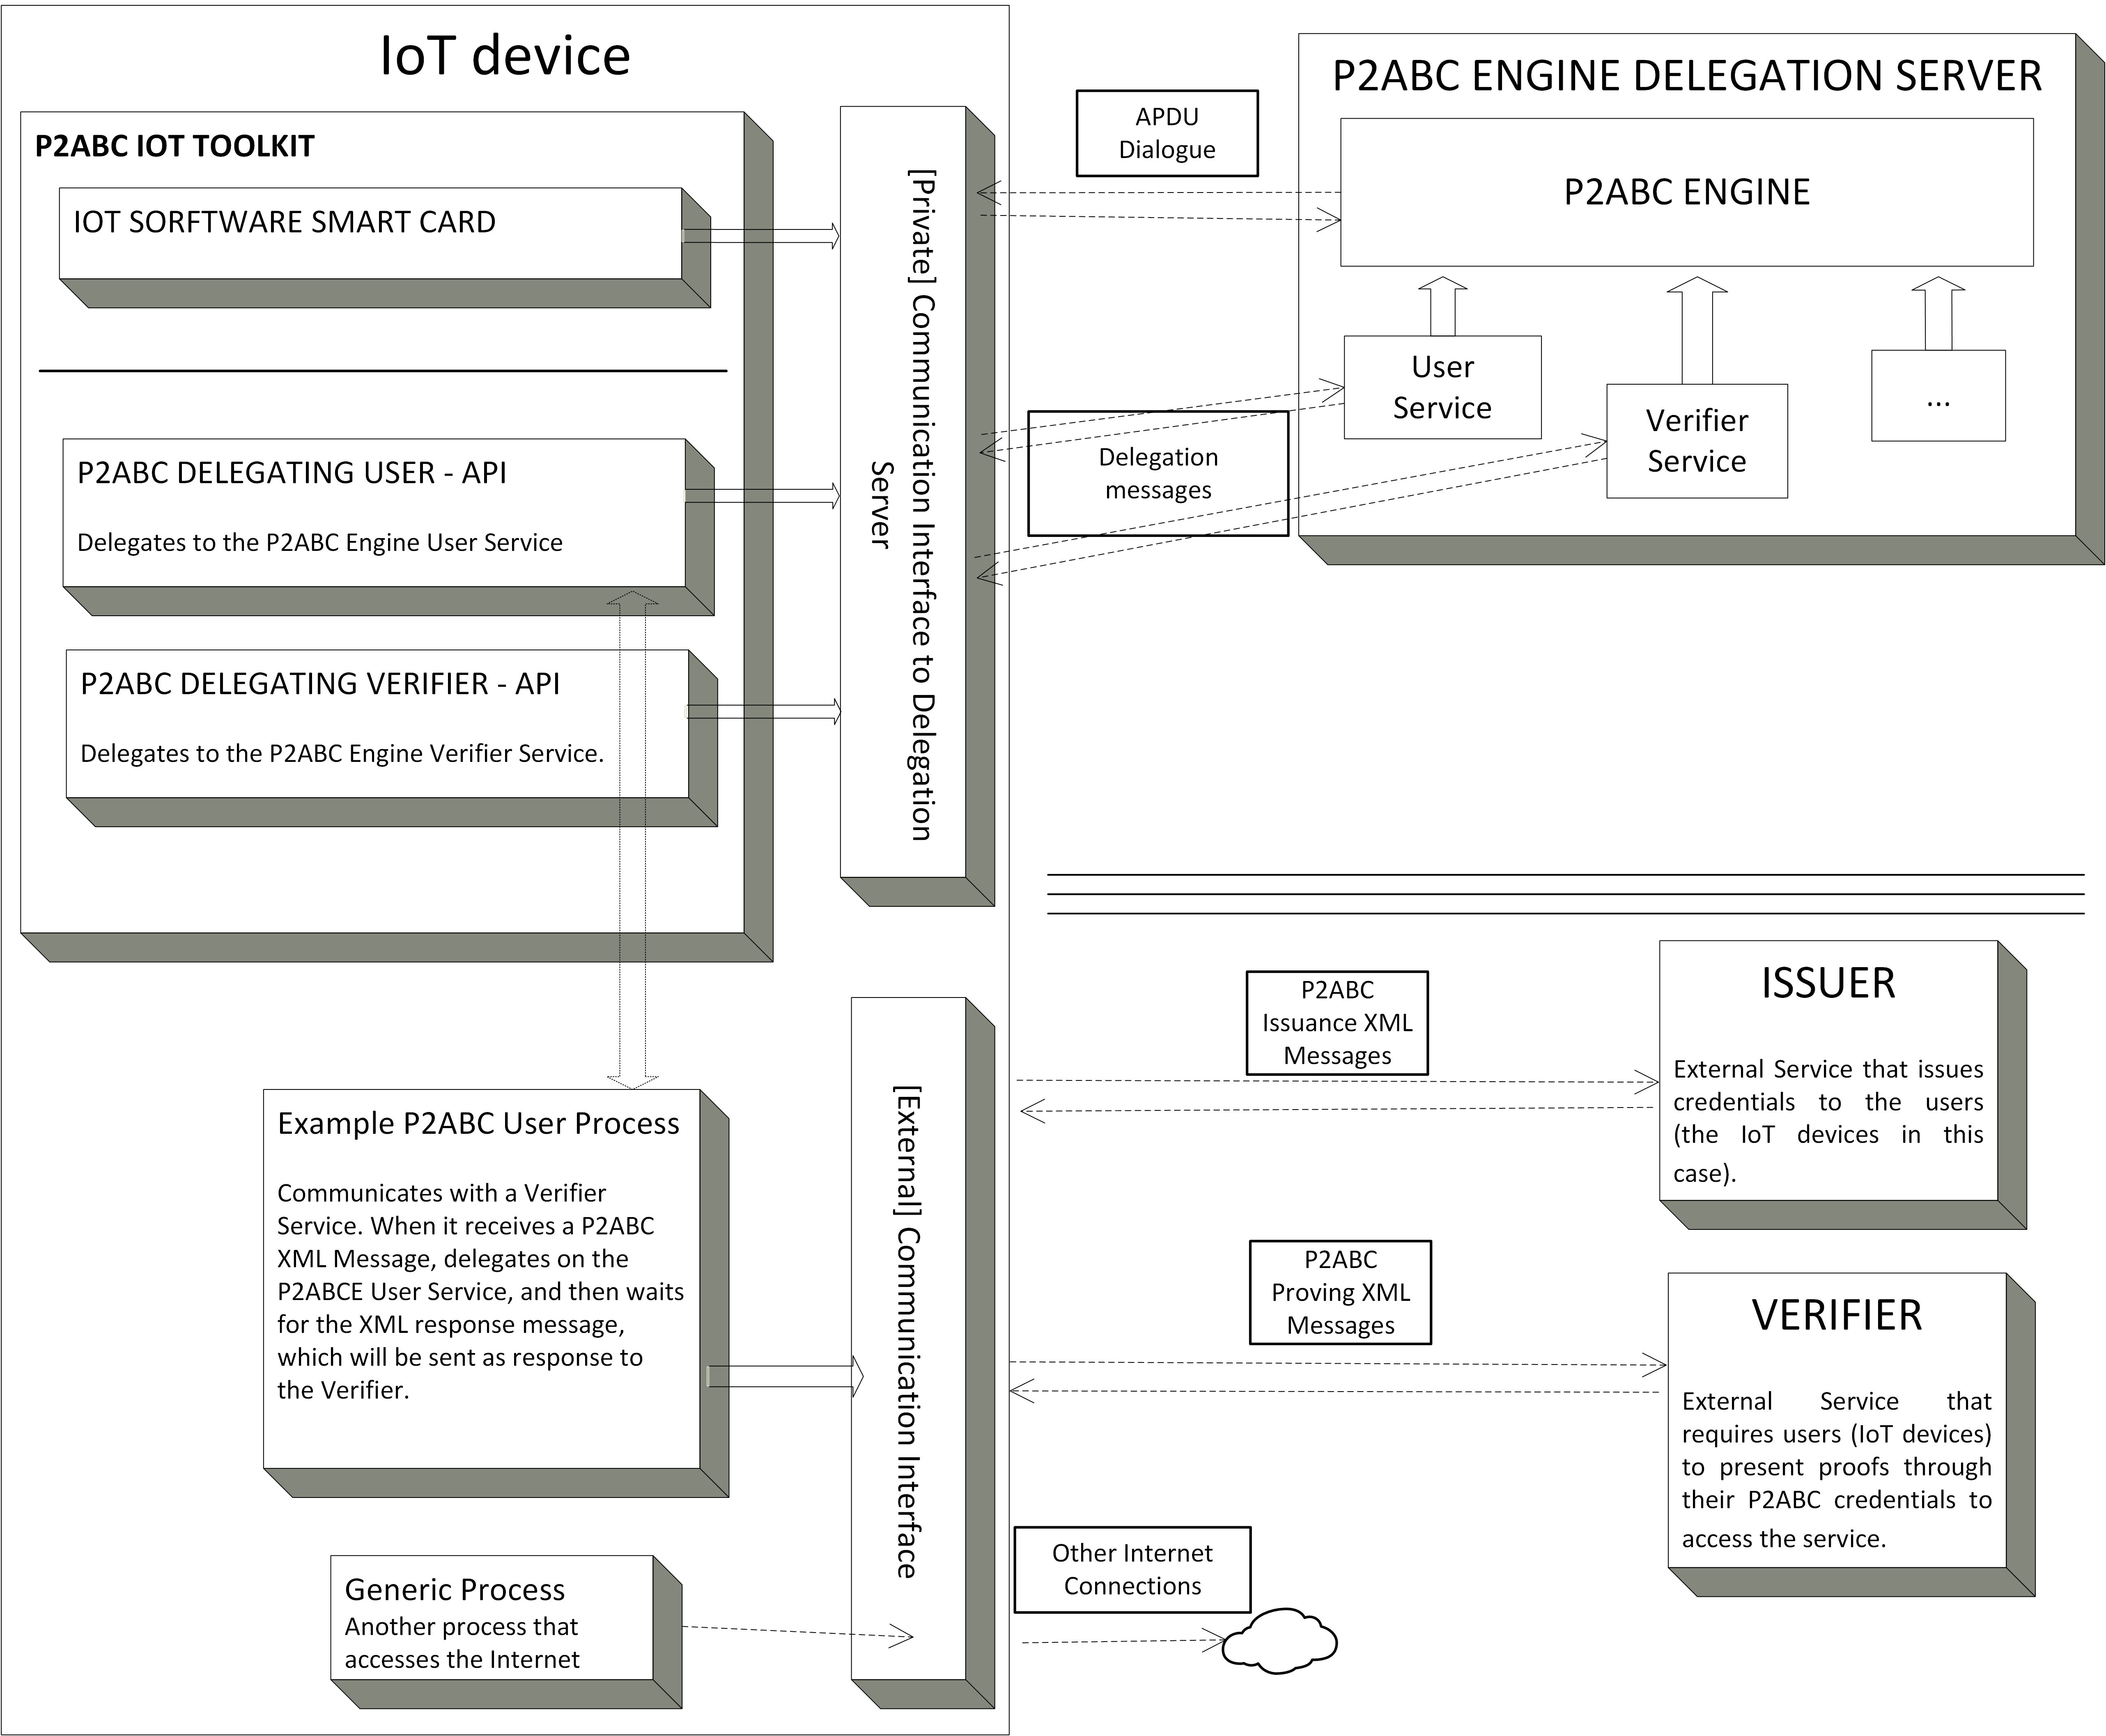
\includegraphics[width=\linewidth]{gfx/P2ABCE-IoT-bw}
	\end{center}
	\caption{Proposed high level Architecture for integrating IoT devices in P2ABCE.}
	\label{fig:P2ABCE-IoT}
\end{figure}

%\begin{figure}[bth]
%	\begin{center}
%		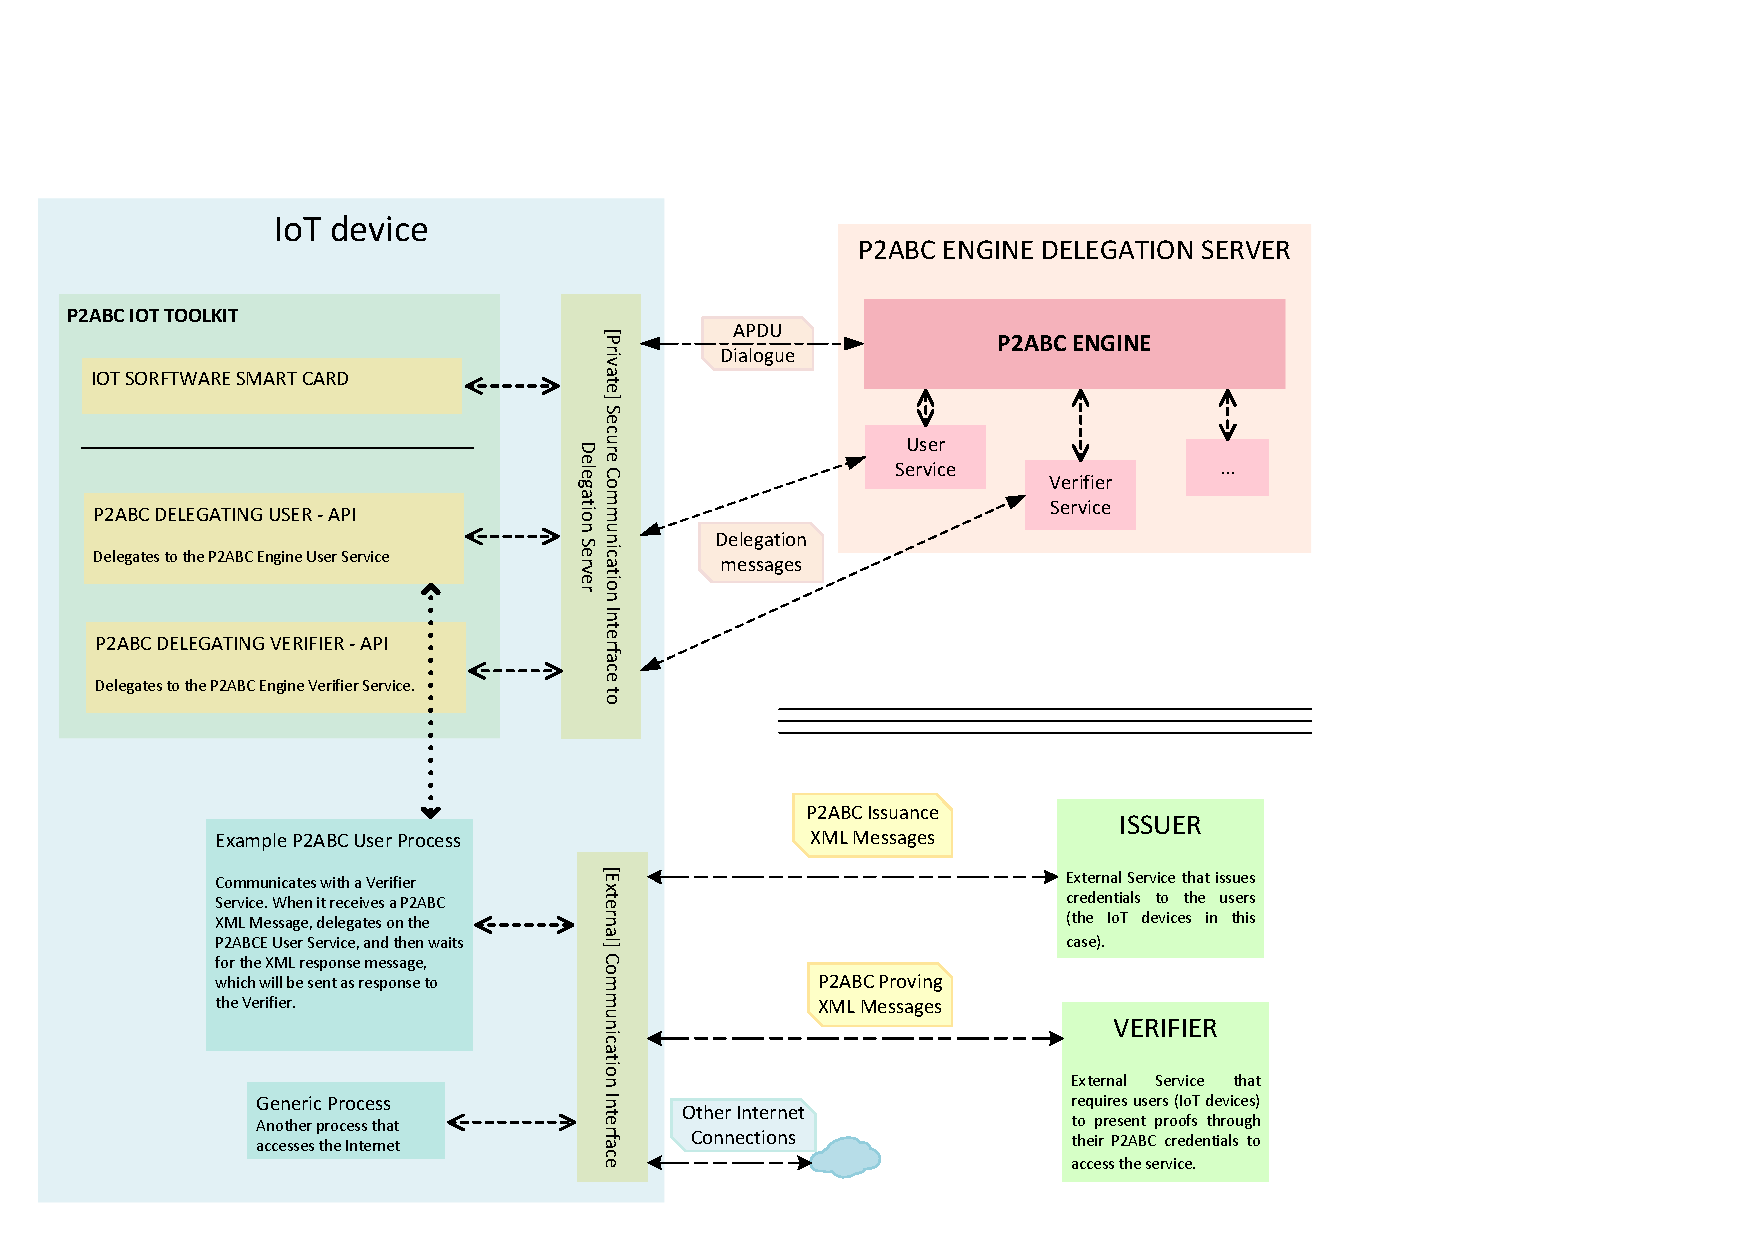
\includegraphics[width=\linewidth]{gfx/P2ABCE-IoT-color}
%	\end{center}
%	\caption{IoT in P2ABCE deployment diagram.}
%	\label{fig:P2ABCE-IoT-color}
%\end{figure}

\hfil


The system will be compounded by the IoT device, the P2ABCE delegation server and the third party P2ABCE actors.

\begin{itemize}
	
	\item \textbf{IoT device}
	
	In \autoref{fig:P2ABCE-IoT} shows our proposed architecture, in which the IoT device is represented with two interfaces, physical or virtual. One allows external communications to other machines, including other P2ABCE actors, that could be on the Internet, a corporate LAN, a M2M overlay network, etc. Through this interface, the P2ABCE XML messages are exchanged as in any other deployment. This allows an IoT device to interact with other actors without special adaptations to the protocol. The other interface allows a secure communication with the delegation server. Both the delegation messages and the APDU Dialogue are transmitted over this interface, making it a point of attack to the system, and we will talk about its security in the delegation process.
	
	The scheme also shows the \textit{P2ABCE IoT Toolkit}. This piece of software includes the IoT Smart Card, and the API for other processes that want to use the P2ABCE system.
	
	The IoT Smart Card is the implementation of a software smart card, listens for APDU Commands from the secure interface and stores securely the credentials and private keys within the device's memory.
	
	The P2ABCE API is an interface for other processes that wish to use the private-preserving environment of P2ABCE. It provides access to every operation available, hiding the delegation process. In the future, if for example the Verification Service is implemented for the IoT device, i.e., there's no need to delegate to other machine to act as a Verifier, then any program using the API won't need to change anything, the toolkit conceals the transition from delegating to native execution.
	
	
	\item \textbf{P2ABCE actors}
	
	If we recall from \autoref{analysisP2ABCE}, the possible roles in the system were the Issuer, the User, the Verifier, the Revocation Authority and the Inspector. All of them use the P2ABCE XML schema in the specification to communicate to each other. Any third party actor will be unaware of the fact that the device is a constrained IoT device that delegates on the P2ABCE server.
	
	
	
	\item \textbf{P2ABCE Delegation Server}
	
	The machine in charge of receiving authorized IoT devices' commands to parse the XML files exchanged and orchestrate the cryptographic operations the IoT smart card must perform.
	
	
\end{itemize}

\hfil

\begin{flushleft}
	\textbf{Delegation process}
\end{flushleft}

Here we describe the computation offloading carried out by the IoT device.  In \autoref{fig:DelegationProving} we show an example of the IoT acting as a User, Proving a Presentation Policy to a third party Verifier.

\begin{enumerate}
	\item Communication with P2ABCE actor.
	
	The IoT device, acting as a User, starts an interaction with another actor, e.g., against an Issuer to obtain a signed credential, or against a Verifier to demonstrate certain property of its attributes in a privacy-preserving way.
	
	\item Delegation to the P2ABCE Server.
	
	Depending on what role the IoT device is acting as, it will delegate in the corresponding service, e.g. User Service. The delegation message must include the XML file, and any parameter required to accomplish the task, like the information on how to communicate with the IoT smart card (listening port, security challenge, etc.).
	
	\item APDU Dialogue (if necessary).
	
	The server may need to send APDU Commands to the IoT smart card to read the credential information or perform cryptographic operations involving private keys, necessarily stored inside the IoT device.
	
	These APDU Commands include a list of 70 different instructions, identified by the APDU INS byte. Some of them manage the smart card, like changing the PIN code, and many are P2ABCE specific, like storing the system cryptographic parameters.
	
	\hfil
	
	\item Server response.
	
	The server may return a status code or a XML file if the first one required an answer from the IoT device, in which case, it will send as response to the third party actor, resuming the communication.
	
\end{enumerate}

\begin{figure}[bth]
	\begin{center}
		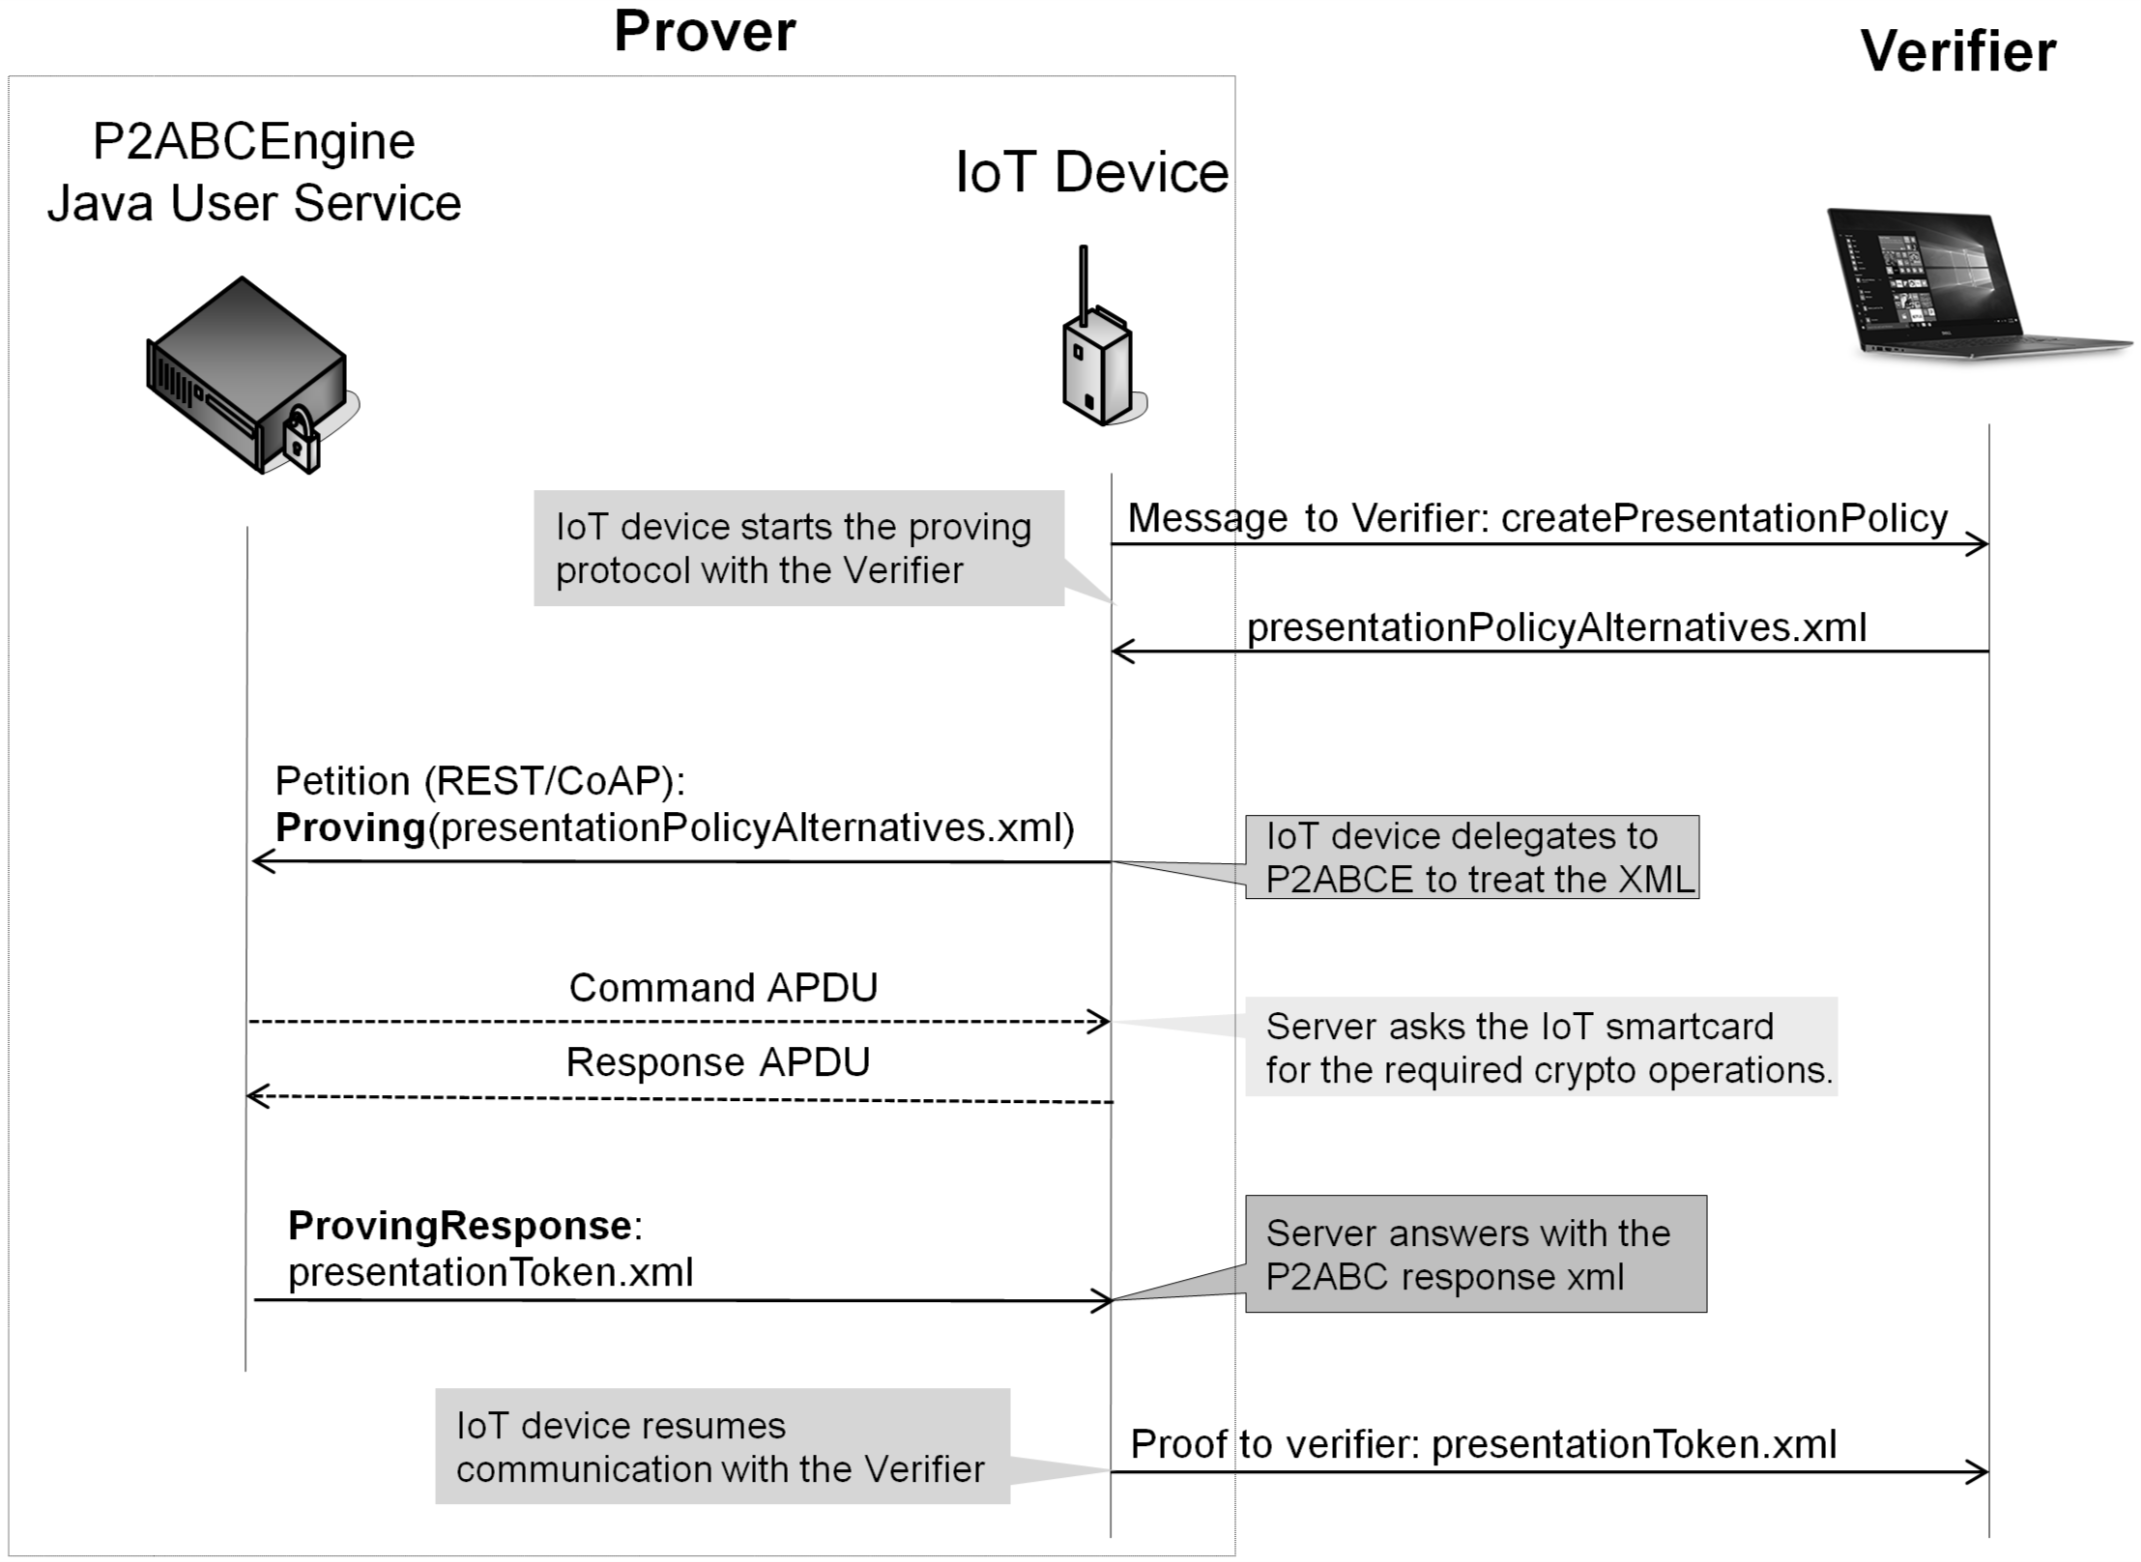
\includegraphics[width=\linewidth]{gfx/UML/DelegationProving}
	\end{center}
	\caption{Designed interactions exchanged during the IoT delegation for P2ABCE Proving operation.}
	\label{fig:DelegationProving}
\end{figure}

Transmissions over the \textit{Server-IoT} channel must be secured in order to avoid attacks like: impersonate the P2ABCE delegation server, having access to the IoT smart card sending the APDU Commands the attacker wishes; delegate as a device on the server but giving the parameters of another device, making the delegation server send the APDU Commands to a victim IoT smart card.


We could use a corporative PKI to issue certificates to the server and devices and configure policies for access control; design a challenge-response system combined with the smart card PIN, like a password and TOTP\footnote{Time-based One-time Password} in a 2FA\footnote{Two-factor authentication} login. We also could connect physically the delegation service through RS-232 serial to the IoT device, securing both physically as we would do with the IoT device on its own, isolating the delegation system from any network attack. This last idea is an approximation to the Arduino Yún\footnote{\url{https://www.arduino.cc/en/Main/ArduinoBoardYun}}, a development board that integrates two microcontrollers, one a typical Arduino with very low resources, and another one running a fork of OpenWrt. The Arduino microcontroller can control the terminal of the more powerful one, using the serial pins as commented before.

As we can see, there are many state of the art solutions for all this threads, therefore, we can assume a secure channel without mentioning a specific solution, providing freedom to choose the most fitting one in a real deployment.


\paragraph{Notes for more constrained devices}

Our architecture is designed for devices that could in a future run a reimplemented version of P2ABCE, that means, the devices could perform more tasks than only running the smart card software and their main purpose process, e.g. recollecting sensor data. But if our target devices are so constrained that can barely run the smart card, they may not be able to handle the XML files because of memory restrictions, like a MSP430\footnote{\url{http://www.ti.com/lsds/ti/microcontrollers-16-bit-32-bit/msp/overview.page}} running Contiki-OS, the microcontroller has between hundred of bytes to tens of kilobytes of memory, making impossible to store multiple XML files in the size range of tens of kilobytes.

In these cases, the delegation in the server goes a step forward, making the server a proxy to communicate with other P2ABCE actors, and the IoT device only acts as a smart card. The IoT device would still act as the User, or any other P2ABCE, role because it orchestrates when and how an interaction with other actor is executed, but the communications would be between the proxy and the third party actor. 



\subsection{Proof of Concept Implementation}
% +Implementation:
% *System:
% 	-Raspbian OS: distro de debian para Raspberry Pi, que se describirá en los tests
% 	-LEDE: ash terminal (shell command interpreter), POSIX, typical hardware, libraries with no hardware aceleration vs smart card MULTOS,
%
% *Delegation
%  -REST as current delegation protocol: curl script bash
%  -BIOSC as current APDU transmission protocol: no security -> no overload.
% *Smart Card
%  
%  -IoT Smart Card software design and implementation notes.
%  -Sequence diagrams. TODO


In this section we present the first PoC implementation, introducing the IoT system where we are going to work, then we will describe the delegation protocols, one for the computation offloading of the IoT device on the P2ABCE server, and another for the transmission of APDU Commands, and finally, we will describe the IoT smart card implementation.



\subsection{IoT system}

We will develop our PoC in Linux based systems in order to avoid complications with firmware specific issues that we are not familiar with. Even so, the linux systems used are aimed for the IoT environment and serve as a starting point for future implementations in more constrained devices or different systems.

In our delegation server we will run Raspbian OS, a distribution based on Debian for the Raspberry Pi. For our IoT device, we will use LEDE, Linux Embedded Development Environment, a distribution forked from OpenWrt, aimed for routers and embedded chips with low resources requirements.



\subsection{PoC Delegation}

As we explained in the design section, the delegation has two steps, the IoT device calling the P2ABCE server to offload the parsing of the XML data, and the P2ABCE server sending APDU Commands to the IoT smart card in the device.


\subsubsection{PoC Delegation to the P2ABCE Server}


Currently P2ABCE offers multiple REST web services to run different roles in P2ABCE system: User Service, Issuer Service, Verification Service, etc. Any third party application that integrates P2ABCE with their system can make use of these services or implement the functionality using the library written in Java, the tool that the REST services actually use.

In this PoC, only the P2ABCE's User Service needed to be modified, because this is the role the IoT device plays. We added the following REST call:
\begin{center}
	\textit{/initIoTsmartcard/{issuerParametersUid}?host=\&port=}
\end{center}
where we communicate the P2ABCE server that an IoT Smart Card is accessible via the IP address \textit{host} and TCP port \textit{port}. Then a new \textit{HardwareSmartcard} object is stored in the P2ABC Engine, but instead of the \textit{javax.smartcardio} Oracle's \textit{CardTerminal} implementation, we use our own \textit{IoTsmartcardio} implementation for the \textit{HardwareSmartcard} constructor, that we will discuss in the following section.


\hfil

%In a real deployment, we would offer a full library with an API for other processes that want to use the P2ABC Engine, which automatizes the boot of the IoT smart card and handles the security policies, like the one we presented in the deployment diagram \ref{fig:P2ABCE-IoT} of the \textit{P2ABCE IoT Toolkit}.

%Now we show some examples of the PoC \texttt{curl} commands, run in the device's terminal, or from a shell script for automation:
%
%\begin{lstlisting}[language=bash]
%$ curl -X POST --header 'Content-Type: text/xml' "http://$DelegationServerIP:9200/user/initIoTsmartcard/http%3A%2F%2Fticketcompany%2FMyFavoriteSoccerTeam%2Fissuance%3Aidemix?host=192.168.3.1&port=8888"
%
%$ curl -X POST --header 'Content-Type: text/xml' -d @firstIssuanceMessage.xml "http://$DelegationServerIP:9200/user/issuanceProtocolStep/" > issuanceReturn.xml
%\end{lstlisting}

%The IoT device will only manage XML as data files to exchange between the third party actor and the P2ABCE delegation service, attaching them in the body of the REST call. In the parameters of the first call we can see the IP and port where the IoT smart card will be listening.



\subsubsection{APDU Dialogue Transmission}


To transmit the APDU messages in our PoC we use a simple protocol, that we will refer as BIOSC (Basic Input Output Smart Card), consisting in one first byte for the instruction.
In the first instruction, we read two header bytes with the length of the APDU Command or Response to receive, followed by said APDU bytes. The message is sent over TCP for a reliable transmission (concept of session, packet retransmission, reordering, etc.). The second instruction serves for closing the TCP socket in the IoT device when the smart card is no longer needed.

We lack any security (authentication or authorization) that a real system should implement. It is vital to authenticate the delegation service, to authorize it to make APDU Commands, and the same with the IoT device, to prevent attacks. But using this method for the transmission of the APDU messages, with only 3 bytes of overhead, helps us in the  benchmarks to measure the real performance of the system.


\hfil


The implementation of this simple protocol is done in Java for the P2abce delegation server and in C for the IoT smart card device.



\hfil

After an analysis of P2ABCE's code, the \texttt{HardwareSmartcard} class implements the \texttt{Smartcard} interface using the package of abstract classes \texttt{javax.smartcardio} to communicate with the physical smart cards. The Oracle JRE implements these package for the majority of smart card manufacturers. For our PoC, we implement the \texttt{javax.smartcardio} package so it transmits the APDUs with BIOSC, making the use of a physical or IoT smart card totally transparent to the \texttt{HardwareSmartcard} class, enhancing maintainability, and following the \textit{expert pattern} from the known GRASP guidelines.

%TODO : optional: diagrama secuencia de P2ABCE, pero si eso solo de la reimplementación de javax.smartcardio y su uso por HardwareSmartcard

\hfil


In our PoC, we implement in \texttt{BIOS.c} the \texttt{main()} function, which reads from a Json file the status of the smart card (keys, credentials, ...), and then opens the TCP socket in the $8888$ port, and loops listening for BIOSC transmissions until an $0xff$ is received. When an APDU Command is sent, it calls the APDU Handler, that we will talk about below.




\subsection{IoT Smart Card Implementation}


After many design decisions in the process to adapt the original ABC4Trust Card Lite code to pure C, working on a MIPS architecture, in this section, we present the current PoC code, most important decisions taken and the execution workflow in the form of sequence diagrams.


\hfil



\subsubsection{Code structure}


We divide the project in three different sections with the objective of enhancing maintainability, improving future changes, ports, fixes, etc.

In \autoref{fig:IoTCScomponents-bw} we show the project's structure. The first section is what could be called as the core of the smart card, the second one the interface for those tools the core needs and that may depend on the target's platform, and finally, the third party libraries, that may be empty if the interfaces implementation doesn't require any.




%\begin{figure}[bth]
%	\begin{center}
%		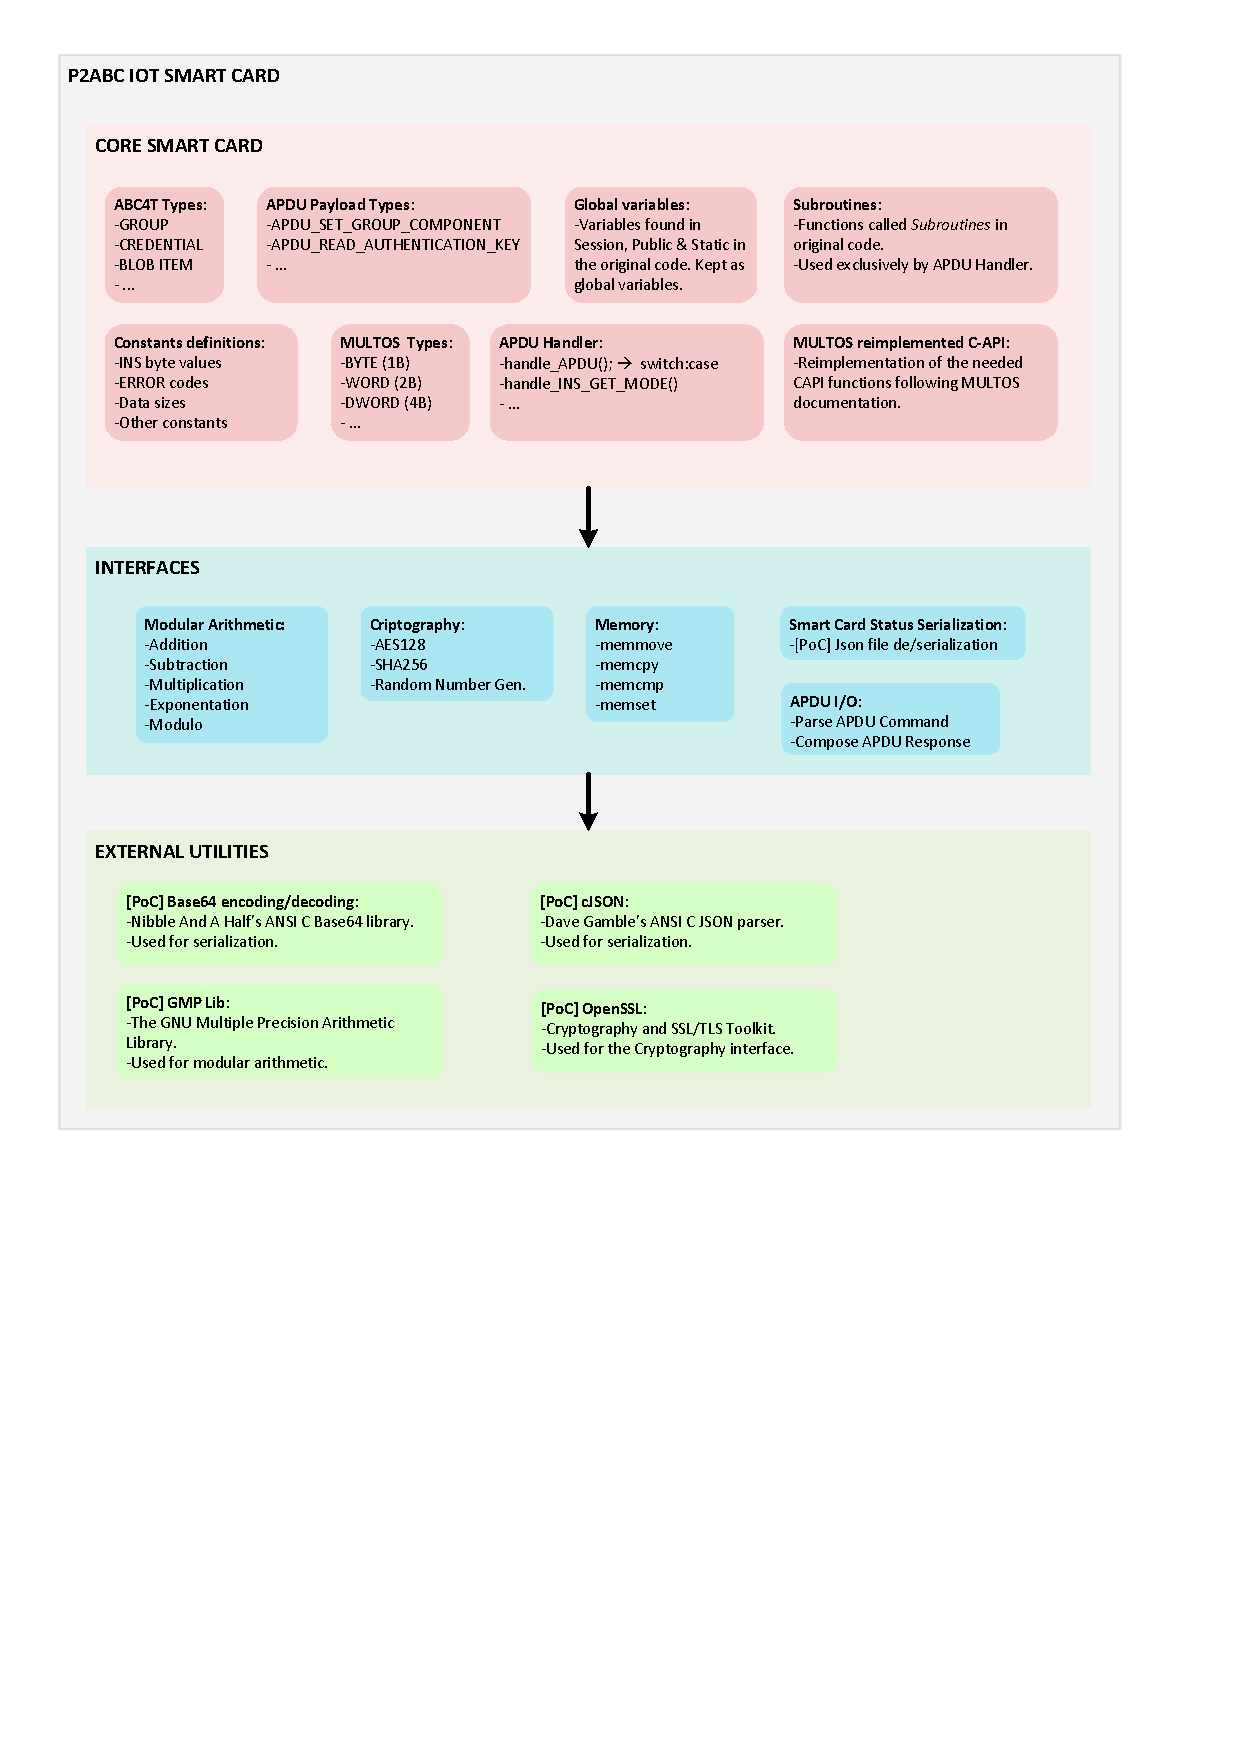
\includegraphics[width=\linewidth]{gfx/IoTCScomponents-color}
%	\end{center}
%	\caption{IoT Smart Card Code Structure.}
%	\label{fig:IoTCScomponents-color}
%\end{figure}

\begin{figure}[bth]
	\begin{center}
		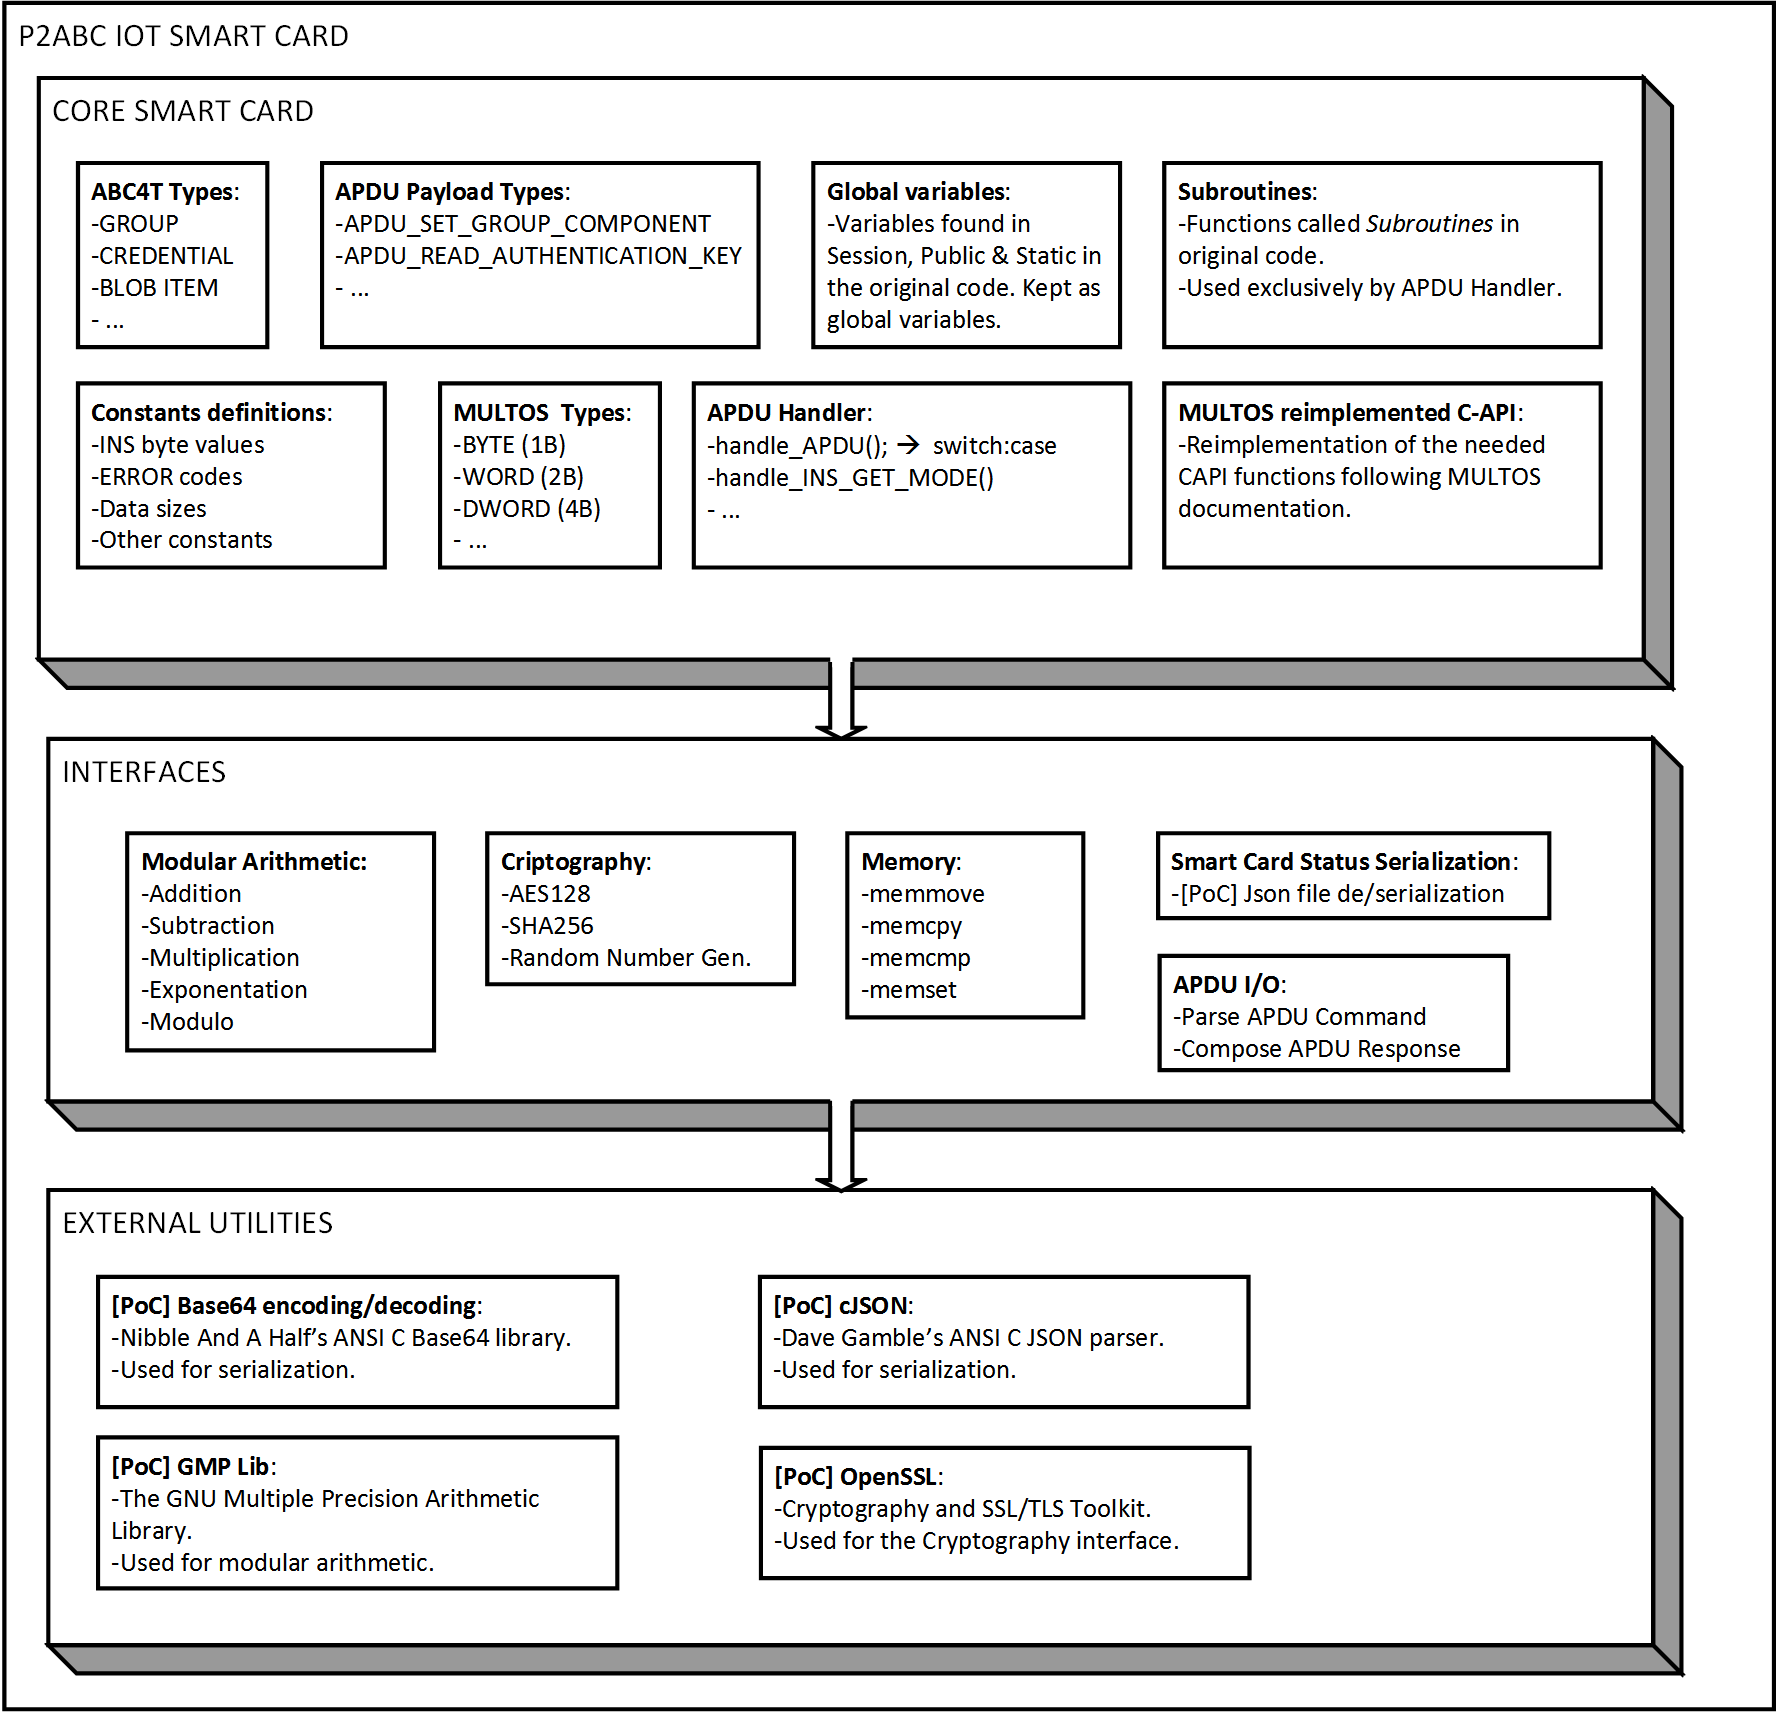
\includegraphics[width=\linewidth]{gfx/IoTCScomponents-bw}
	\end{center}
	\caption{IoT Smart Card Code Structure.}
	\label{fig:IoTCScomponents-bw}
\end{figure}


\hfil

\textbf{Core smart card}
\hfil

The smart card logic lies in this section, the concepts of APDU Commands, what instructions are defined for P2ABCE smart cards, and how to process them and generate proper APDU Responses.

Most of the original ABC4Trust Card Lite's code has been reused in this section, e.g., all the global variables and custom data type definitions, the APDU Command handling and auxiliary subroutines.

However, the ABC4Trust's code heavily depended on the MULTOS platform for the input and output of data, modular arithmetic, memory management, and AES128 and SHA256 cryptographic operations. Therefore, we reimplement the used MULTOS functions following the documentation, adapting it in some cases for \textit{expanded functionality} when needed, like in \cite{vullers2013efficient} when they noted that MULTOS' \texttt{ModularExponentiation}  function does not accept exponents larger than the modulus size, so they implemented \texttt{SpecialModularExponentiation}.

In MULTOS, to reduce the memory usage, the MULTOS compiler does not apply padding between variables in the data structures, i.e., data structure alignment\footnote{\url{https://en.wikipedia.org/wiki/Data_structure_alignment}}.
This affects the inherited ABC4Trust's code because of the use of \texttt{memcpy} to copy zones of memory from one address to another. The problem is the code copies multiple variables in one \texttt{memcpy} call, because, for example, the APDU Command payload includes multiple data, and instead of copying one variable at a time, the \texttt{struct} is defined with the same order and copies everything at once.

The temporal solution is to use \texttt{struct \_\_attribute\_\_((\_\_packed\_\_))} to ask a GCC compiler to not use padding in the structs, but this is not standard, neither a good practice. A deeper refactorization of the code is needed where the hidden copies of variables are made explicit, letting the compiler manage the memory layout.



\textbf{Interfaces}\hfil

To reimplement some of the MULTOS functions, we needed to use some libraries, so we defined a facade to isolate the implementation of the core smart card from our different options, that could vary depending on the hardware or the system used by the IoT device.

The use of a facade lets us, for example, change the implementation of modular arithmetic with a hardware optimized version, or a future more lightweight library, or our very own software implementation using the same data types that the core uses, minimizing the data usage.

The interfaces defined can be organized in 5 groups (see \autoref{fig:IoTCScomponents-bw}), depending on their purpose: Modular Arithmetic, Cryptography, Memory Management, Serialization, APDU Parsing.


\textbf{External utilities}\hfil

In our PoC, we use two ANSI C libraries, for base64 and JSON, and two shared libraries available in as packages in LEDE, GMPLib and OpenSSL. These libraries use dynamic memory and offer more functionality than we need, although they are a good tool in this PoC, future versions should use more lightweight solutions, optimized fo the target device.

\hfil

The \textit{interfaces} and \textit{external utilities} sections  allow that the project is easily ported to specific targets without modifying the smart card logic.



\subsubsection{Execution workflow}

The sequence diagram from \autoref{fig:sequenceBIOSC} shows the execution of the PoC IoT smart card.



\begin{figure}[bth]
	\begin{center}
		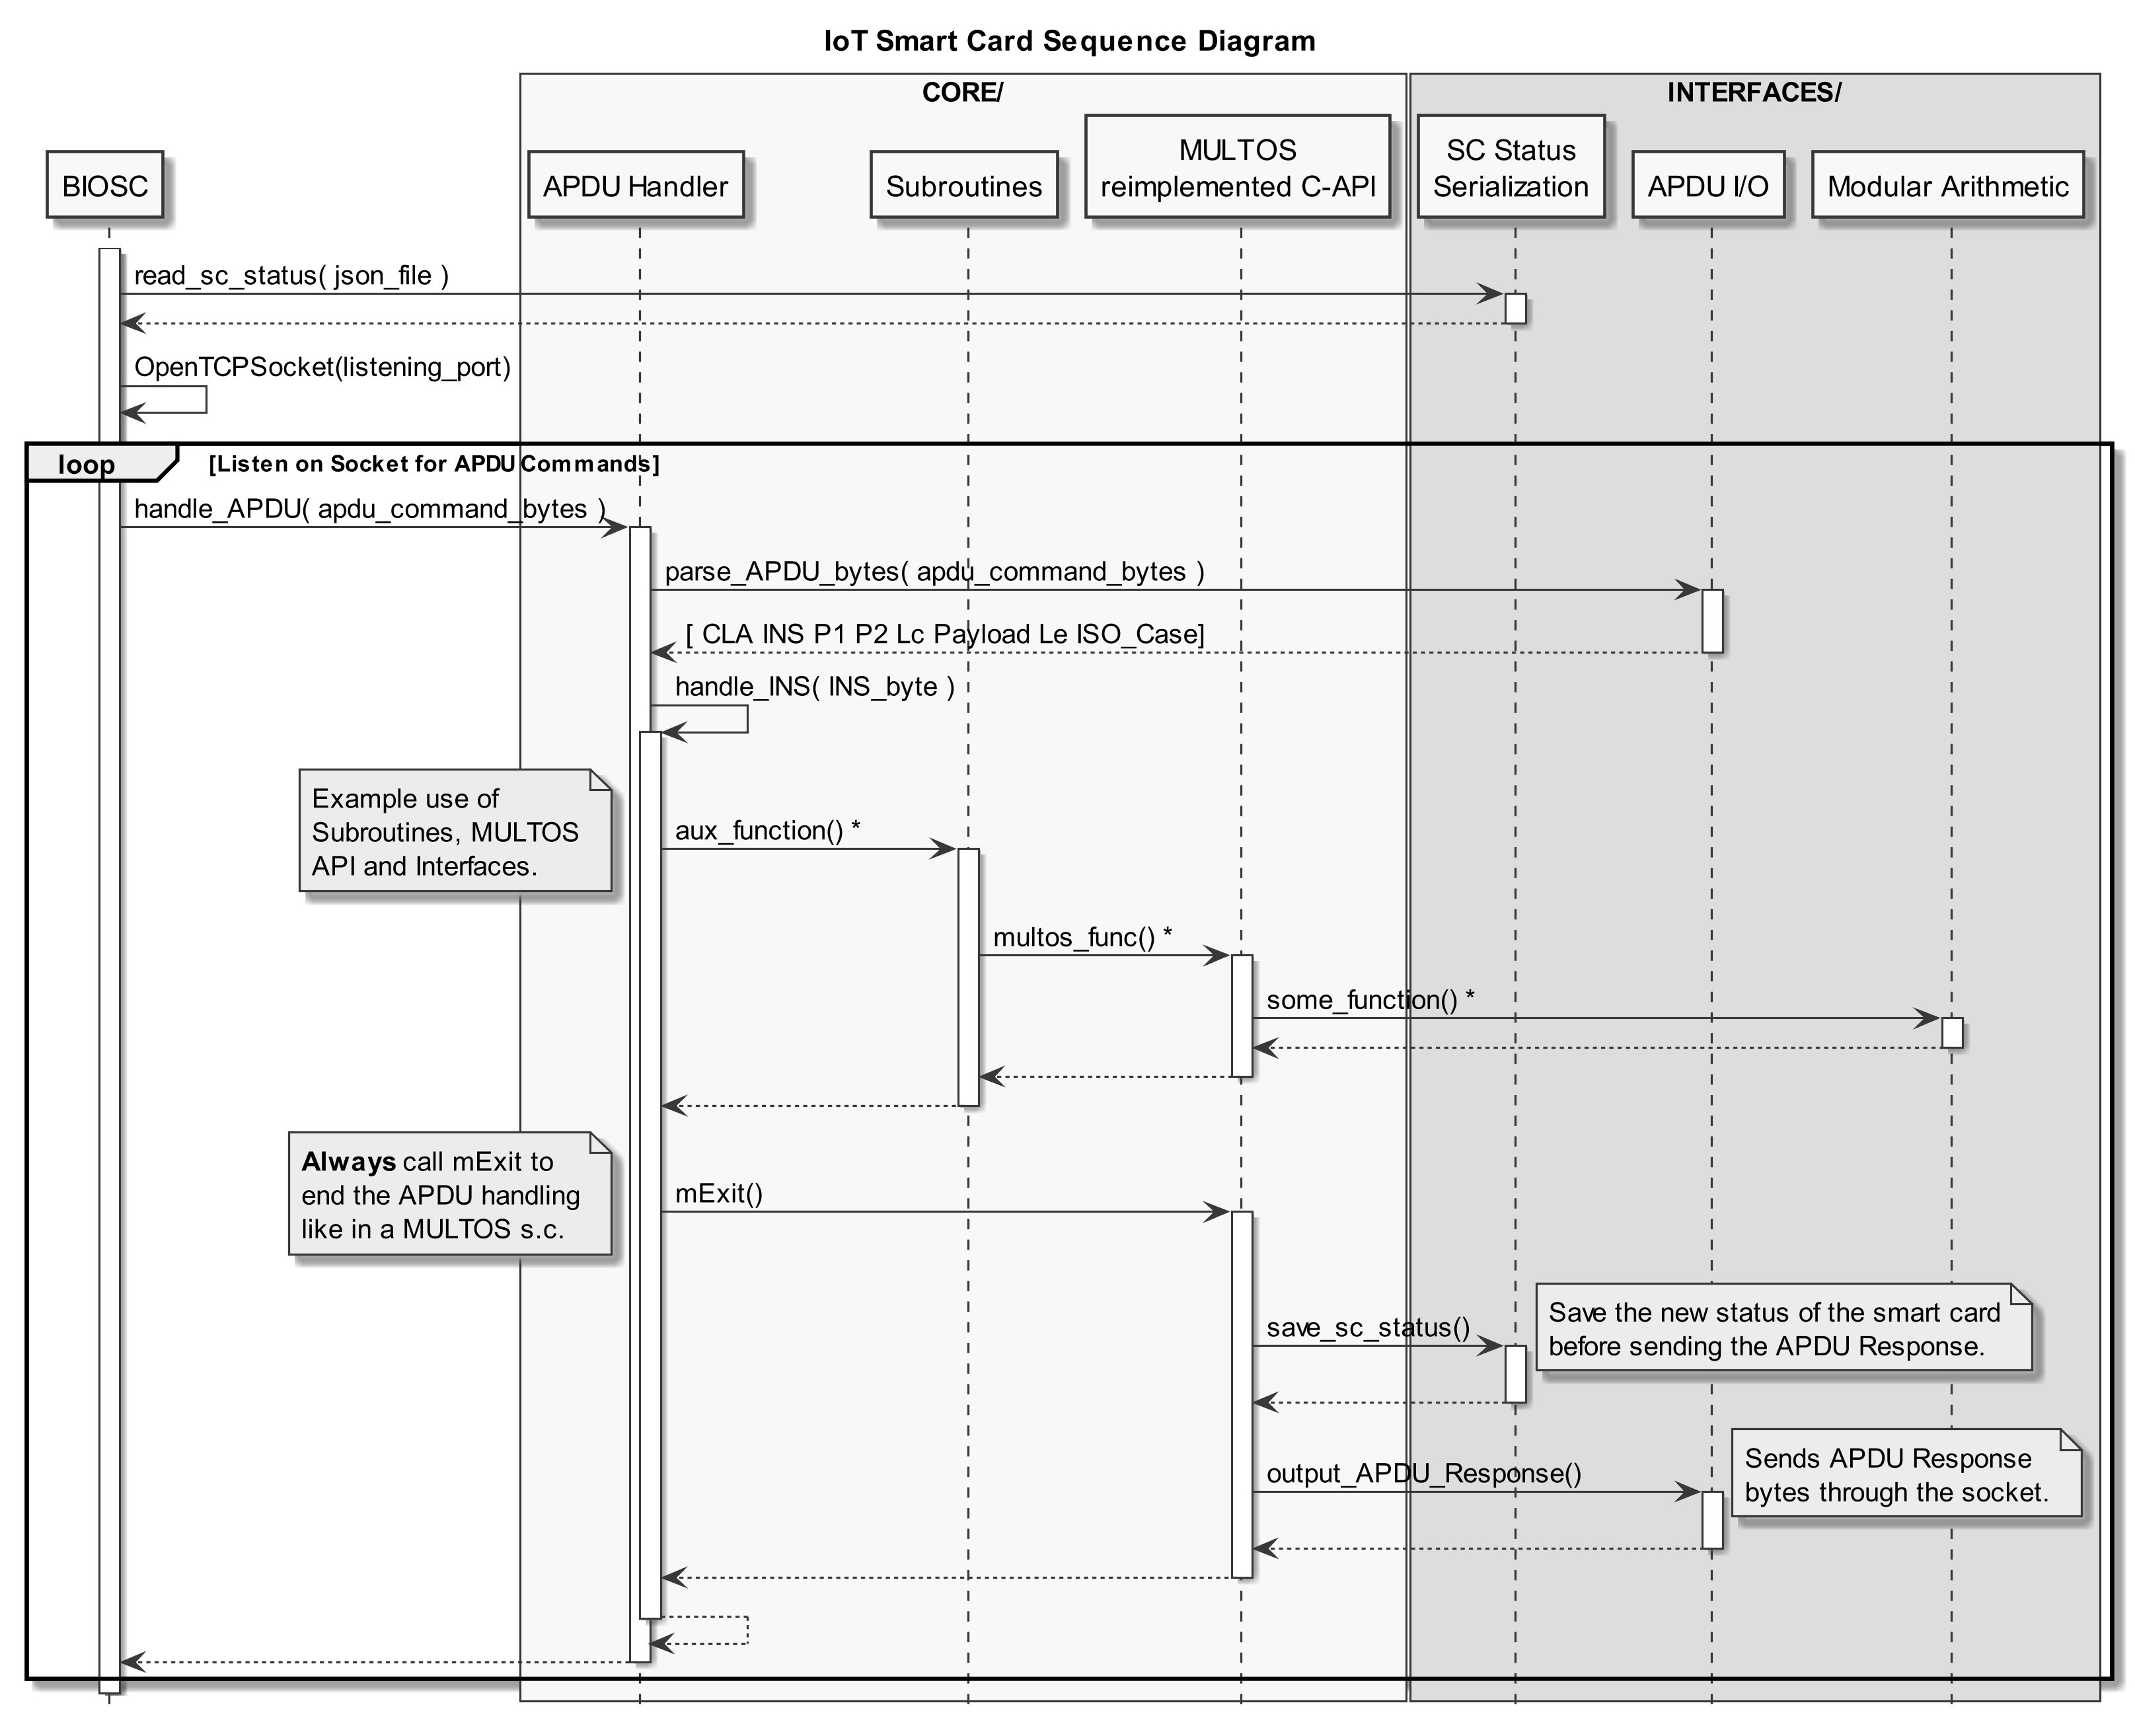
\includegraphics[width=\linewidth]{gfx/UML/sequenceBIOSC}
	\end{center}
	\caption{IoT Smart Card Sequence Diagram.}
	\label{fig:sequenceBIOSC}
\end{figure}



The program starts with the \texttt{main} function in BIOSC, that deserializes the status from the Json file, and listens on a loop for APDU Commands from the delegation server.

Every time an APDU Command arrives, it calls the function \texttt{handle\_APDU()} with the raw APDU bytes. The Handler calls the APDU I/O interface to parse the bytes, storing in global variables the APDU structure. Using a \texttt{switch-case} expression on the \texttt{INS} byte, the Handler calls an \textit{Instruction handler} function.

Inside this function, it may call multiple functions from the Subroutines, that may call MULTOS C-API functions, Which in turn may use an interface to perform its functionality.

Finally, every instruction handler must end, before the \texttt{return;} expression, with a call to \texttt{mExit}. This reimplemented MULTOS function will save the current status of the smart card and send the APDU Response back to the delegation server.

After returning from the functions \texttt{mExit}, instruction handler and APDU handler, the program listens again from the socket.



%************************************************
\section{Validation and Performance Evaluation}\label{ch:validation}
%************************************************

In this section, we will describe the deployment of three testing scenarios: a laptop, a Raspberry Pi 3, and a Omega2 IoT device with the Raspberry Pi 3 as the delegation server. We will measure and compare the results to determine if the proposed solution is feasible or must be submitted to revision.

\subsection{Testbed description}

First, we shall describe the example Attribute Based Credential system in use. Then, the hardware we will use in our benchmarking.

\subsubsection{P2ABCE setting}

To test the correct execution of the \textit{IoT smart card}, we will use the ABC system from the tutorial in the P2ABCE Wiki\footnote{\url{https://github.com/p2abcengine/p2abcengine/wiki/}}. It is based on a soccer club, which wishes to issue VIP-tickets for a match. The VIP-member number in the ticket is inspectable for a lottery, ie. after the game, a random presentation token is inspected and the winning member is notified.

First the various entities are \textbf{setup}, where several artifacts are generated and distributed. Then a ticket credential containing the following attributes is issued:

\begin{verbatim}
First name: John
Last name: Dow
Birthday: 1985-05-05Z
Member number: 23784638726
Matchday: 2013-08-07Z
\end{verbatim}

During \textbf{issuance}, a \textit{scope exclusive pseudonym} is established and the newly issued credential is bound to this pseudonym. This ensures that the ticket credential can not be used without the smart card.

Then \textbf{presentation} is performed. The \textit{presentation policy} specifies that the member number is inspectable and a predicate ensures that the matchday is in fact $2013-08-07Z$. This last part ensures that a ticket issued for another match can not be used.

The ticket holder was lucky and his presentation token was chosen in the lottery. The presentation token is therefore inspected.


\hfil

\subsubsection{Execution environment}

First we will execute the test in our development machine (laptop). After asserting that the services work as expected, we then run the test in a Raspberry Pi 3\footnote{\url{https://www.raspberrypi.org/products/raspberry-pi-3-model-b/}}, exactly like in the laptop. Finally, we will deploy the IoT smart card in a Omega2\footnote{\url{https://docs.onion.io/omega2-docs/omega2.html}} and the delegation services in the Raspberry Pi 3. After every test, we checked that the issuing and proving were successful, in case a cryptographic error appeared in the implementation. 

A downside of using the Omega2 is the lack of hardware acceleration for cryptographic operations, unlike the MULTOS applications, because the smart cards hardware and MULTOS API include support for such common operations in smart cards.



\paragraph{The network} In our third scenario, the Raspberry Pi 3 and the Omega2 will talk to each other over TCP. This implies possible network delays depending on the quality of the connection. The Raspberry Pi 3 is connected over Ethernet to a switch with WiFi access point. The Omega2 is connected over WiFi n to said AP. To ensure the delay wasn't significant, we measured 6000 APDU messages, and the results show that the mean transmission time is less than half a millisecond per APDU. From our analysis of the tests we conclude that the network time is negligible compared to the rest of the computations.



\subsection{Results}

After 20 executions for each scenario (laptop, RPi3, Omega2+RPi3), we take the means and compare each step of the testbed.

It is worth noting that during the test, the measured use of the CPU showed that P2ABCE does not benefit of parallelization, therefore, it only uses one of the four cores in the laptop and Raspberry Pi 3.

To test the network, we sent six thousand APDUs to the Omega2, but instead of calling the \textit{APDU handler}, the Omega2 responded with the same bytes back. This way, the Omega2 only performed the simple BIOSC protocol, reading from and writing to the TCP socket.
The APDUs had multiple sizes, taken from the most common APDUs logged in during a successful execution. The test showed that our network speed was around $0.014$ ms per byte.


\paragraph{The setup}\hfil

The first step of our testbed. The Omega2 doesn't intervene until the creation of the smart card, therefore, the times measured in the second and third scenarios are practically identical.

\begin{figure}[bth]
	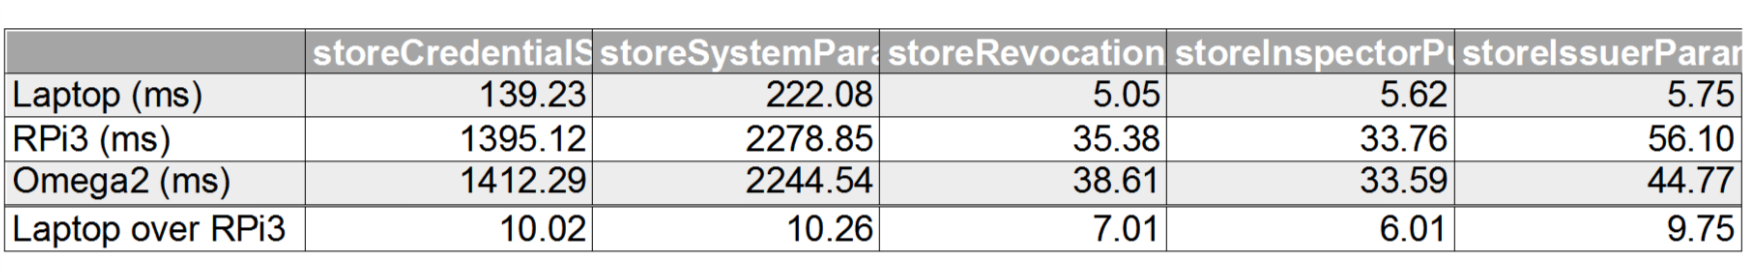
\includegraphics[width=\linewidth]{gfx/graphics/setuptable}
	\caption{Setup times (milliseconds). Times and relative speedup}
	\label{fig:setup:graph}
\end{figure}

%\begin{figure}[bth]
%	\caption{Setup times (milliseconds). Comparison graph}
%	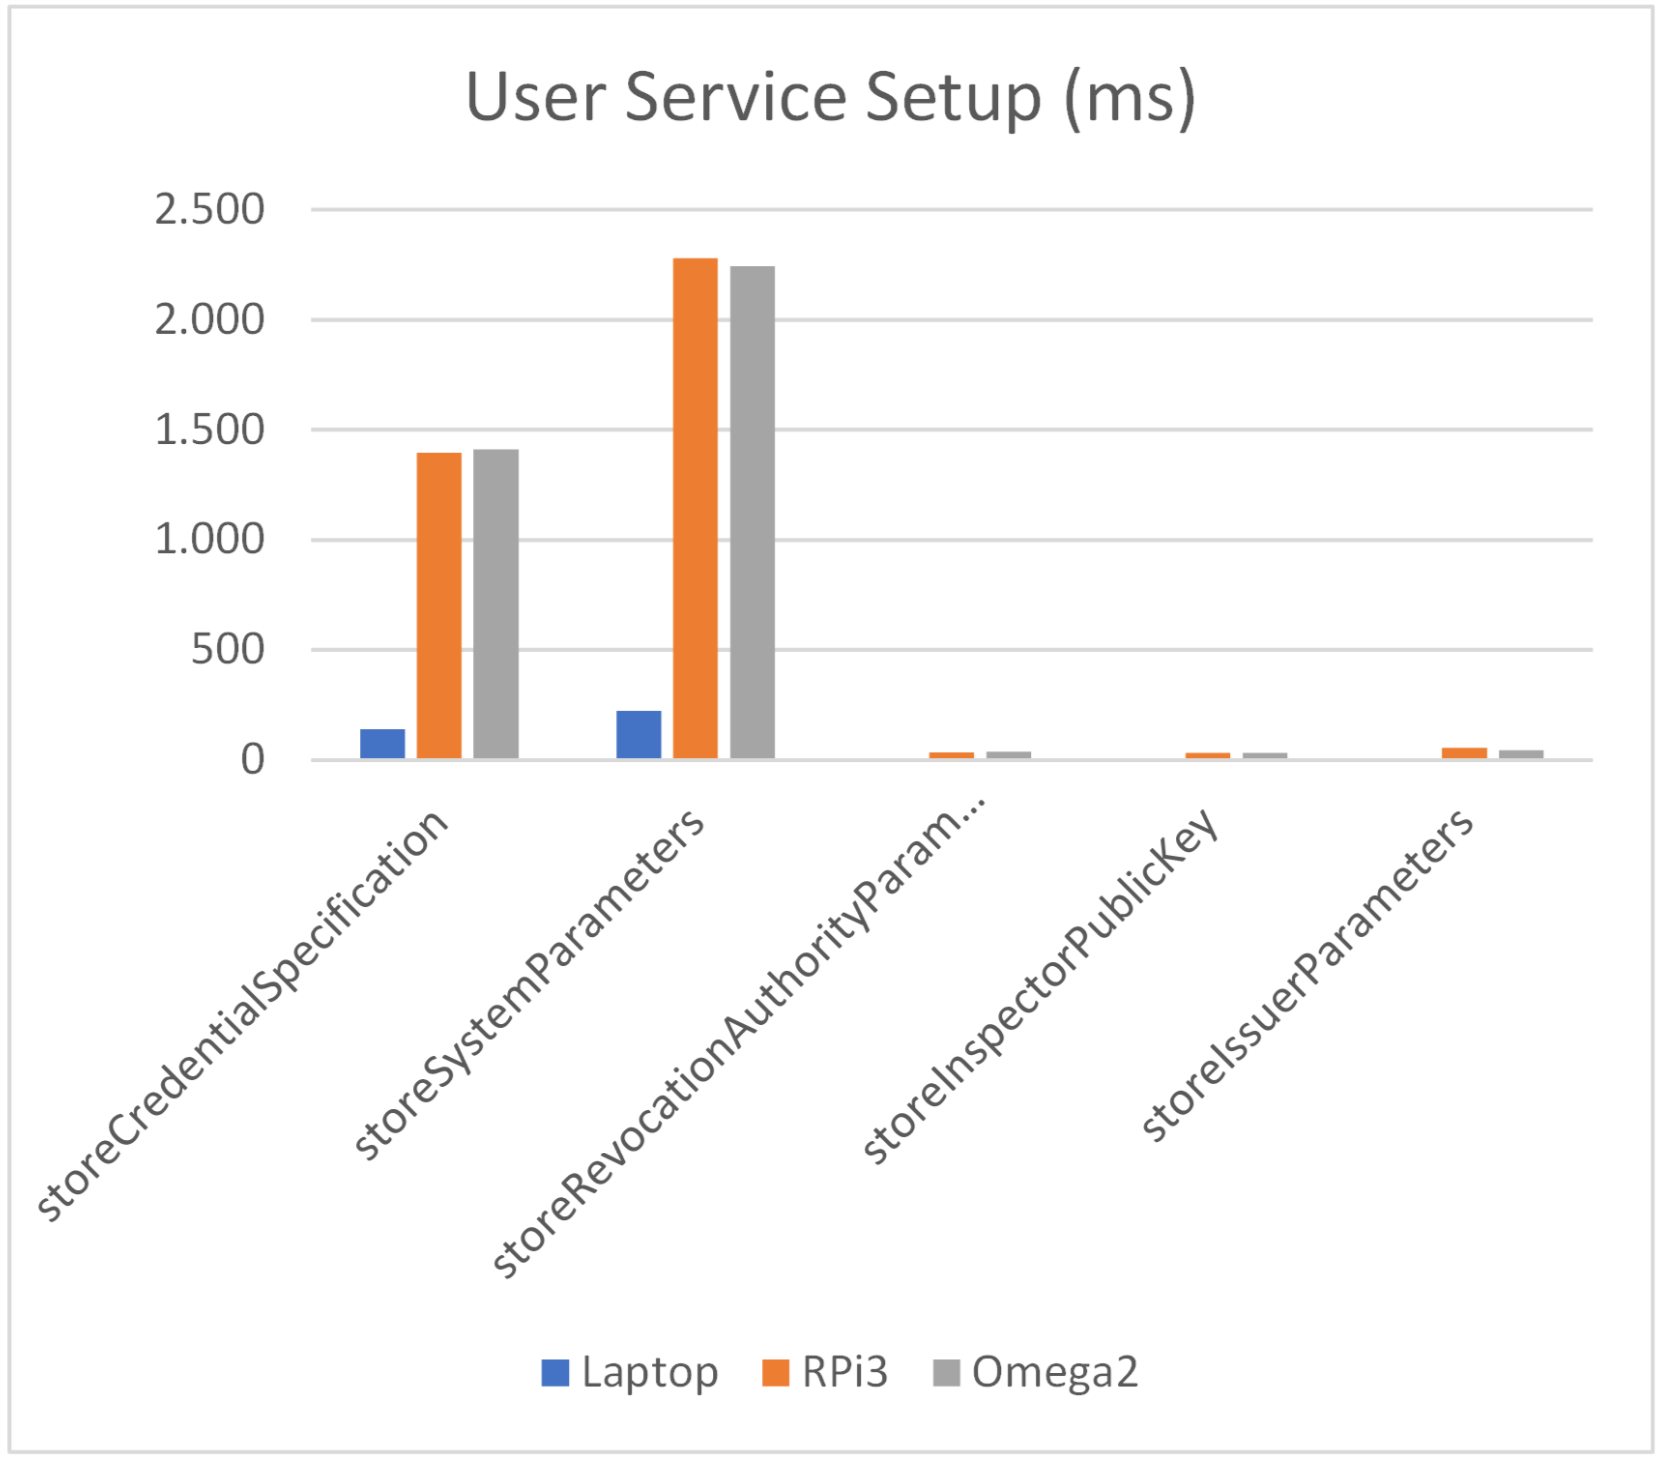
\includegraphics[width=0.8\linewidth]{gfx/graphics/setup}
%	\label{fig:setup:graph2}
%\end{figure}

As we can see in \autoref{fig:setup:graph}, the laptop is about ten times faster than Raspberry Pi 3, but considering that the highest time is less than two and a half seconds, and that the setup is done only once, this isn't a worrisome problem.

\paragraph{Creation of the smart card}\hfil

Here we create a \textit{SoftwareSmartcard} or a \textit{HardwareSmartcard} object that the User service will use in the following REST calls.

The REST method to create a \textit{SoftwareSmartcard} is $/createSmartcard$, and to create a \textit{HardwareSmartcard}, using the \textit{IoTsmartcardio} implementation, we use $/initIoTsmartcard$. This operation is done only once per device, and includes commands from the creation of the PIN and PUK of the smart card, to storing the system parameters of P2ABCE, equivalent to the previous setup step.


\begin{figure}[bth]
	\caption{Create smart card times (seconds). Times and relative speedup}
	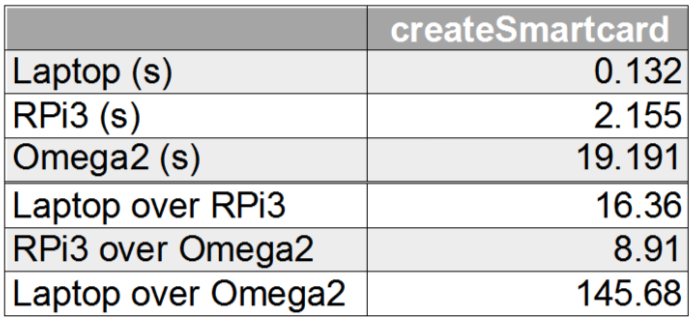
\includegraphics[width=0.7\linewidth]{gfx/graphics/createSCtable}
	\label{fig:createSmartCard:graph}
\end{figure}

%\begin{figure}[bth]
%	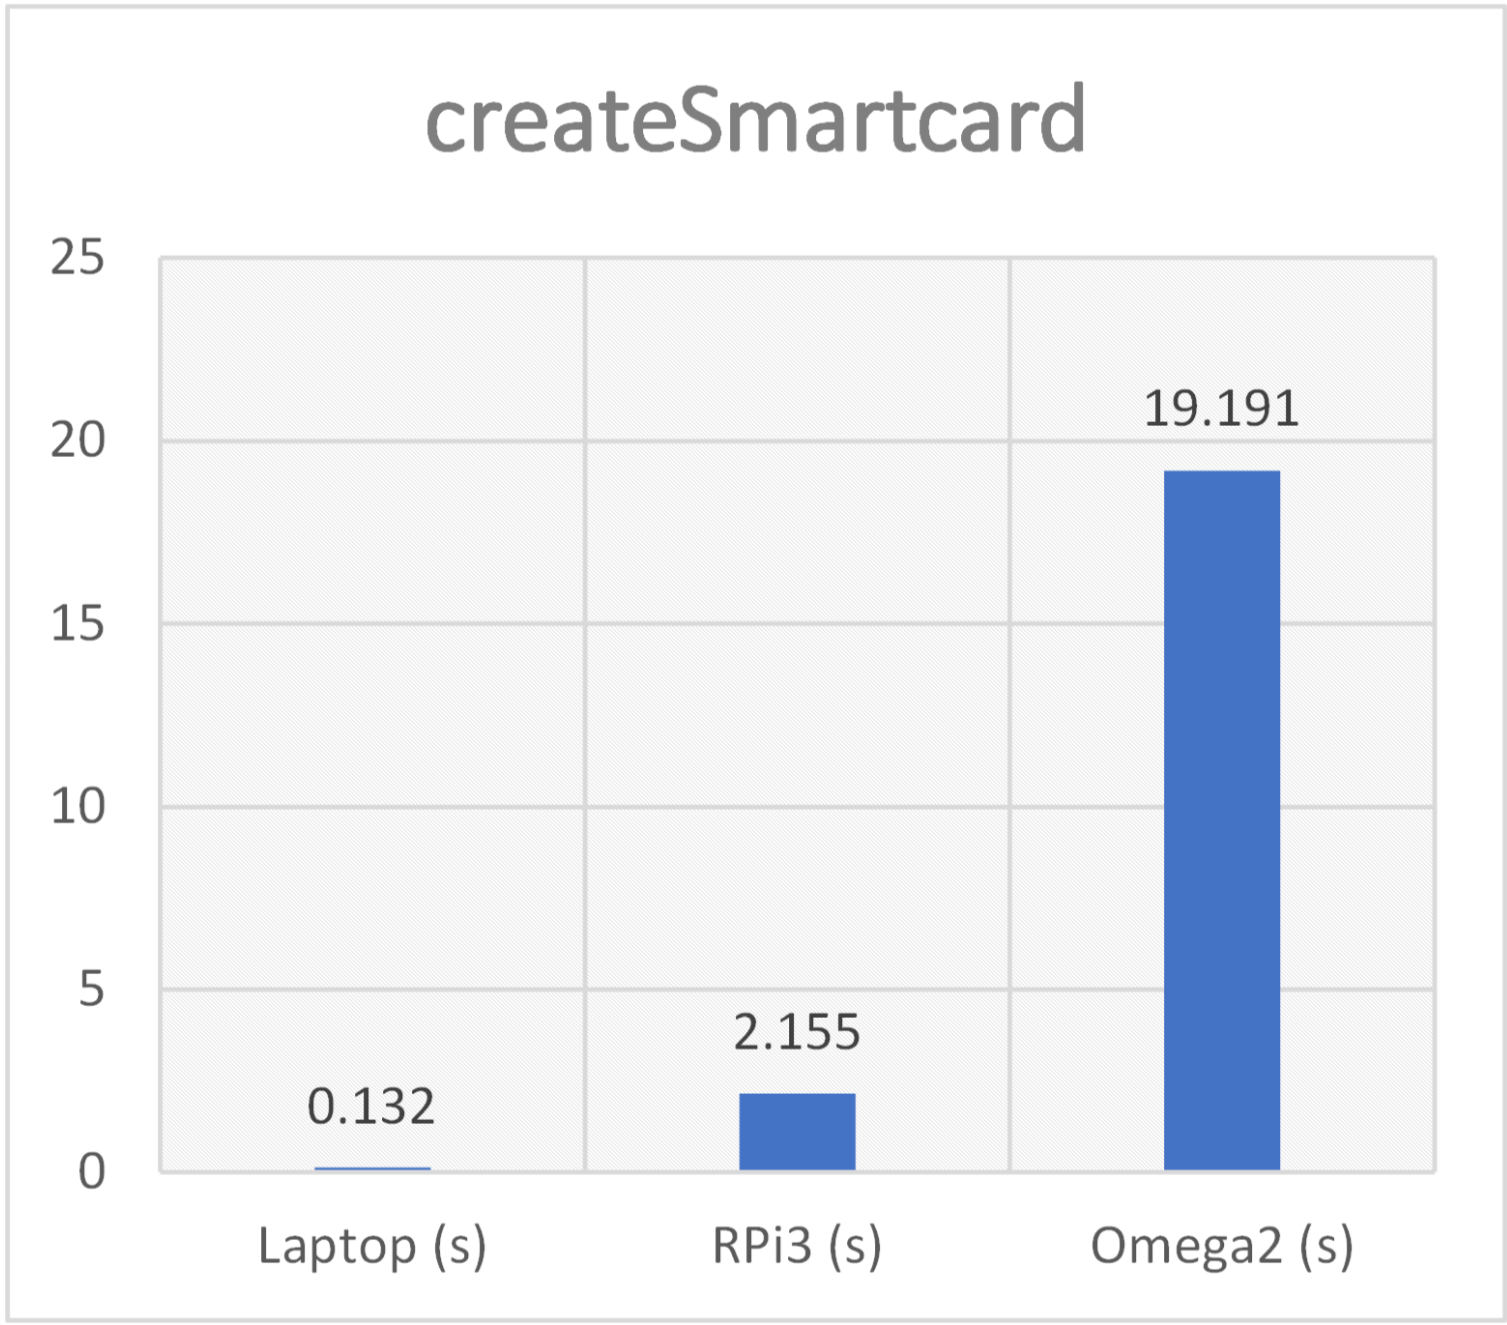
\includegraphics[width=0.8\linewidth]{gfx/graphics/createSC}
%	\caption{Create smart card times (seconds). Comparison graph}
%	\label{fig:createSmartCard:graph2}
%\end{figure}


From \autoref{fig:createSmartCard:graph} we see that the RPi3 is about 16 times slower than the laptop in the creation of the \textit{SoftwareSmartcard}, but almost 9 times faster than the setup of the smart card in the Omega2 using APDUs. This gives us that the laptop is 145 times faster than the combination of RPi3 and Omega2 in our IoT deployment.
But looking at the times, this process lasts up to 20 seconds, making it something feasible.

This is the first interaction between the RPi3 and the IoT smart card running in the Omega2. To setup the smart card 30 APDU Commands, and their respective Responses, are exchanged, with a total of $1109$ bytes. From our network benchmark, using TCP sockets, the delay in the transmission is only around 15 and 20 ms, negligible, as we said, compared to the almost 20 seconds the operation lasts.


\paragraph{Issuance of the credential}\hfil

Our credential will have 5 attributes and key sizes of 1024 bits, as specified during the setup process.

The three delegation steps and the REST method called are:

\begin{center}
	\begin{tabular}{l|l}
		First issuance protocol step & $/issuanceProtocolStep$ \\
		Second issuance protocol step  & $/issuanceProtocolStepUi$ \\
		\textit{(end of first step for the User)} & \\
		Third issuance protocol step & $/issuanceProtocolStep$ \\
		\textit{(second step for the User)}  & \\
	\end{tabular}
\end{center}


%\begin{figure}[bth]
%	\begin{center}
%		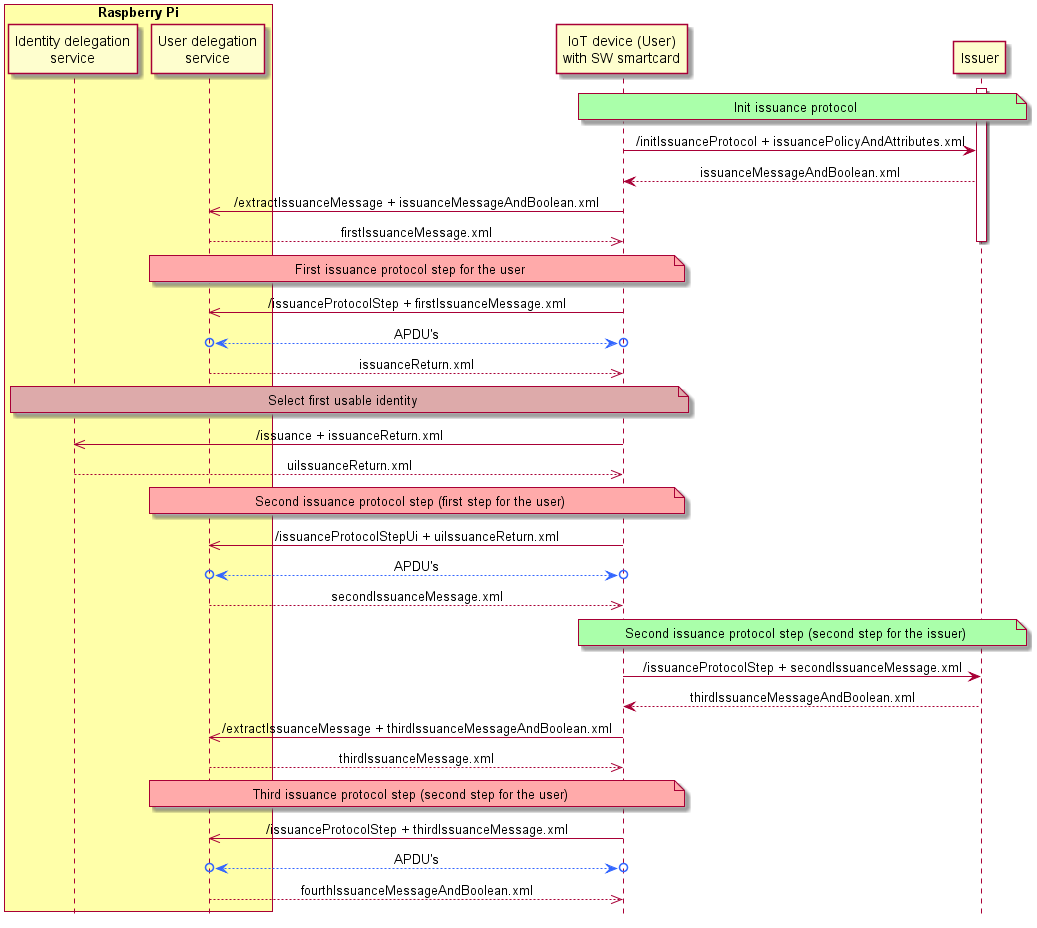
\includegraphics[width=\linewidth]{gfx/UML/IssuanceInteraction}
%	\end{center}
%	\caption{Issuance interaction.}
%	\label{fig:IssuanceInteraction}
%\end{figure}



As we can see, the three REST calls to the delegation User service involve communication with the smart card. There are 45 APDU Commands in total, $3197$ bytes exchanged, that would introduce a latency of 45ms in the network, negligible.


\begin{figure}[bth]
	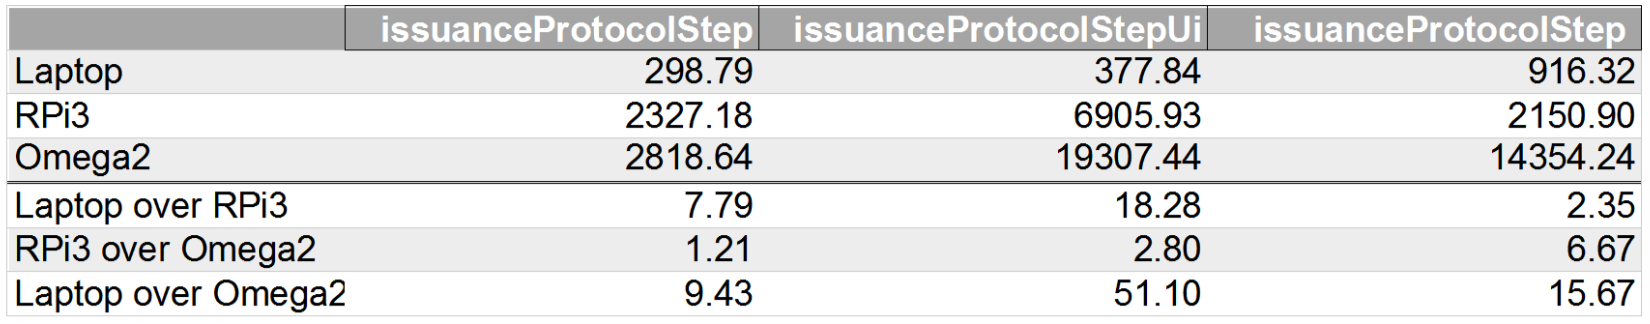
\includegraphics[width=\linewidth]{gfx/graphics/issuancetable}
	\caption{Issuance times (milliseconds). Times (ms) and relative speedup}
	\label{fig:issuance:graph}
\end{figure}

%\begin{figure}[bth]
%	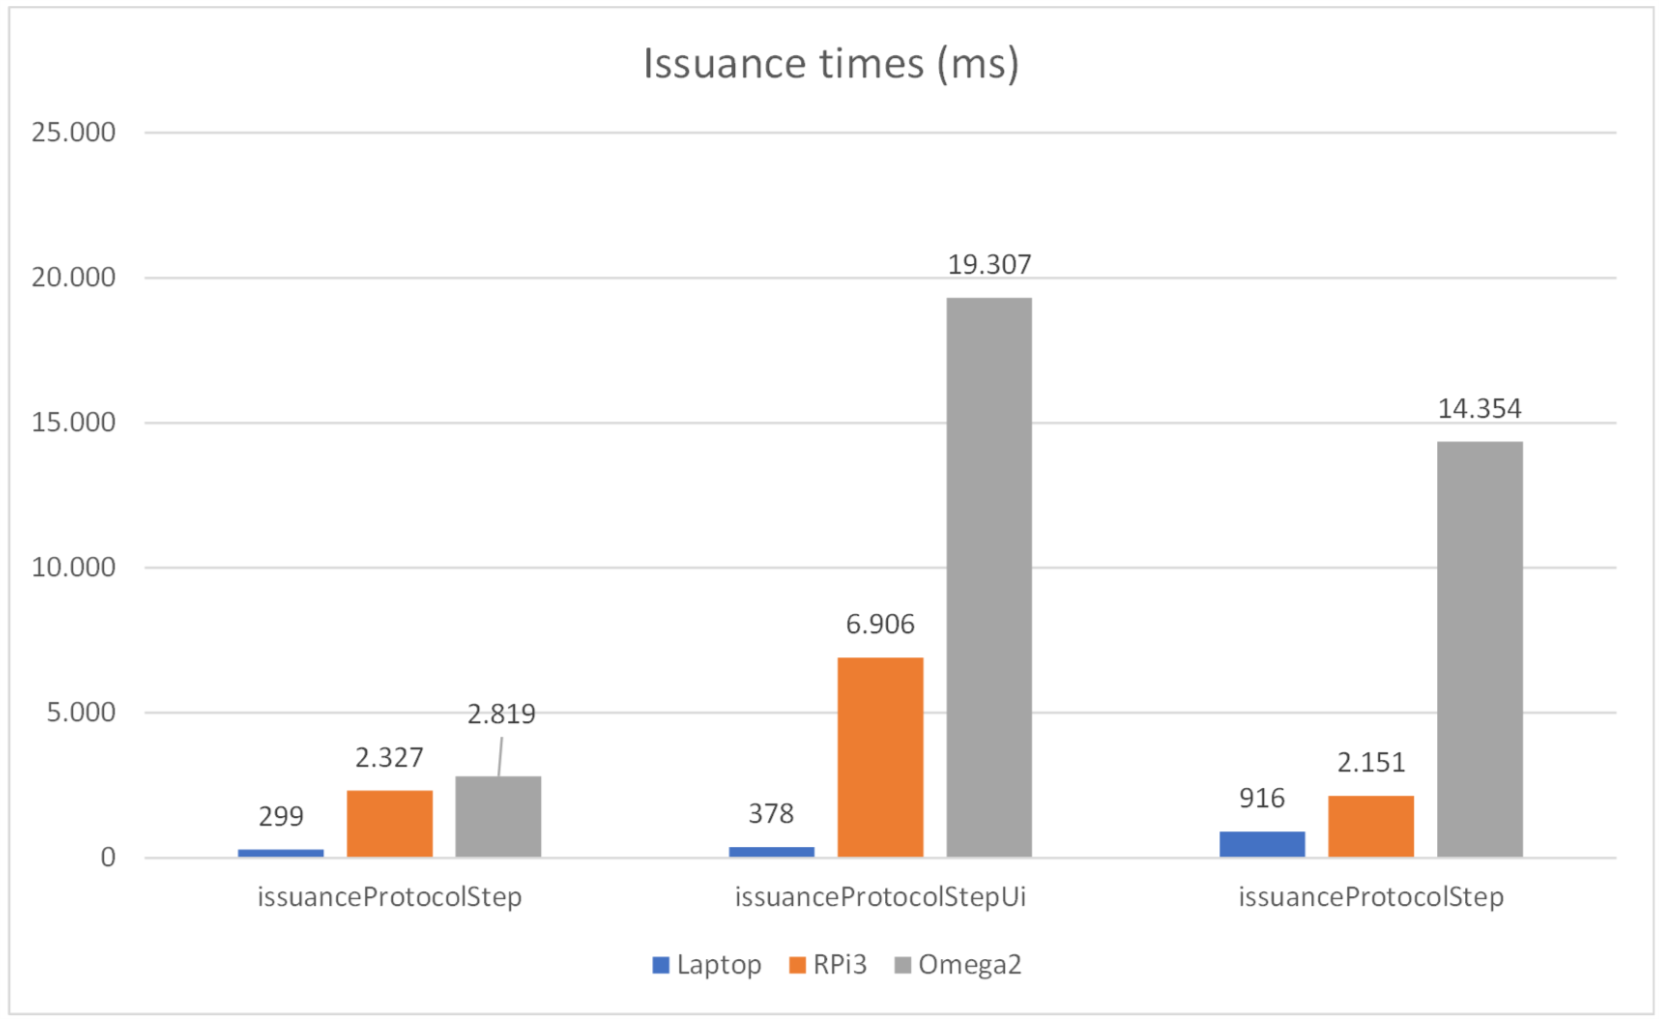
\includegraphics[width=\linewidth]{gfx/graphics/issuance}
%	\caption{Issuance times (milliseconds). Comparison graph}
%	\label{fig:issuance:graph2}
%\end{figure}

In \autoref{fig:issuance:graph} we have the times spent in each REST call. The laptop shows again to be many times faster than the other two scenarios, but the times are again feasible even for the IoT environment.

Lets compare the Raspberry Pi 3 and the Omega2 executions. There is a correlation between the number of APDU Commands needed in each step with the increment in time when using the IoT smart card, that is, how much the delegation server.

The first one only involved one APDU, with $33$ bytes total (Command and Response), and times are almost identical. The second call needed $34$ APDUs, with $1623$ bytes, and the increase in time is around tree times slower than the RPi3 on its own. The third call used $20$ APDUs, $1541$ bytes, and makes the IoT scenario almost 7 times slower.

The analysis shows where there are more cryptographic operations involving the Omega2, and because the amount of data exchanged is minimal, the difference in processing power between Omega2 and Raspberry Pi 3 is clear.



\paragraph{Presentation token}\hfil

The final step of the test involves a Prove, or Presentation in P2ABCE, where the Verifier sends the User or Prover the Presentation Policy, and the User answers with the Presentation Token, without more steps. 
%In \autoref{fig:ProvingInteraction}, using the same colors as in the Issuance interaction, we can see the delegation messages done by the Omega2.

To ensure that all the process was successful, it's enough to check if the Verifier and the Inspector returned XML files, accepting the prove, or an error code. Of course, every execution measured in the test was successful.

The APDU Commands and Responses pairs sent are $28$ in total, with $1939$ bytes, giving us about $27$ms of delay in the network transmission.



%\begin{figure}[bth]
%	\begin{center}
%		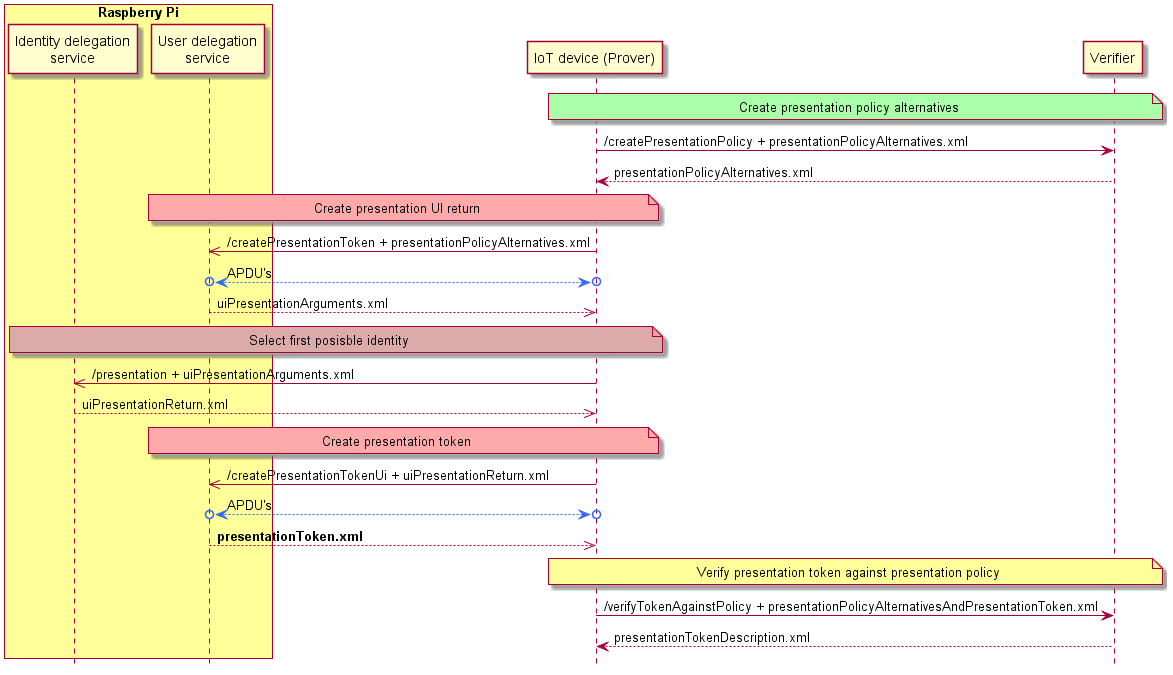
\includegraphics[width=\linewidth]{gfx/UML/ProvingInteraction}
%	\end{center}
%	\caption{Proving interaction.}
%	\label{fig:ProvingInteraction}
%\end{figure}



Again, as shown in \autoref{fig:proving:graph}, there is a correlation between the number of APDU Commands used, the work the IoT smart card must perform, and the time measured. The $20$ APDU Commands in the first call make the IoT deployment almost $8$ times slower than the Raspberry Pi 3; but with only $8$ APDU Commands, the second one is less than $1.5$ times slower.

Nonetheless, it's significant the difference in performance between the laptop and the Raspberry Pi 3 in the last REST call, more than $40$ times slower, even using the \textit{SoftwareSmartcard}.


\begin{figure}[bth]
	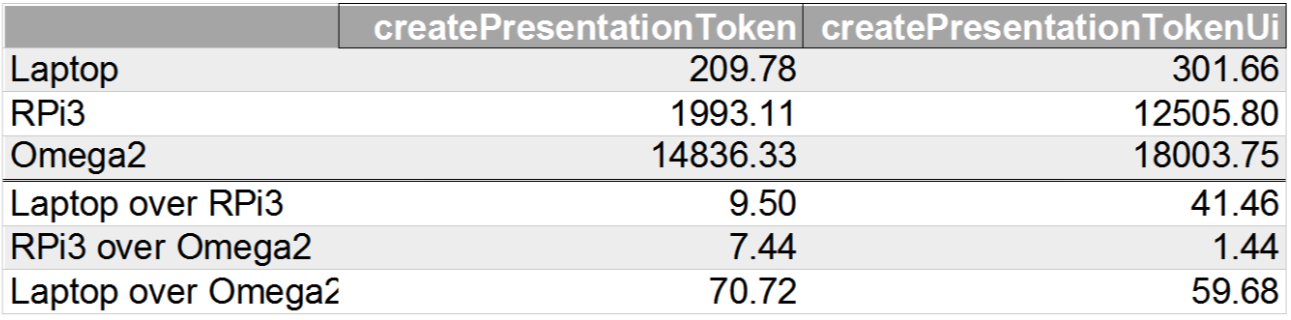
\includegraphics[width=.8\linewidth]{gfx/graphics/provingtable}
	\caption{Proving times (milliseconds). Times (ms) and relative speedup}
	\label{fig:proving:graph}
\end{figure}

%\begin{figure}[bth]
%	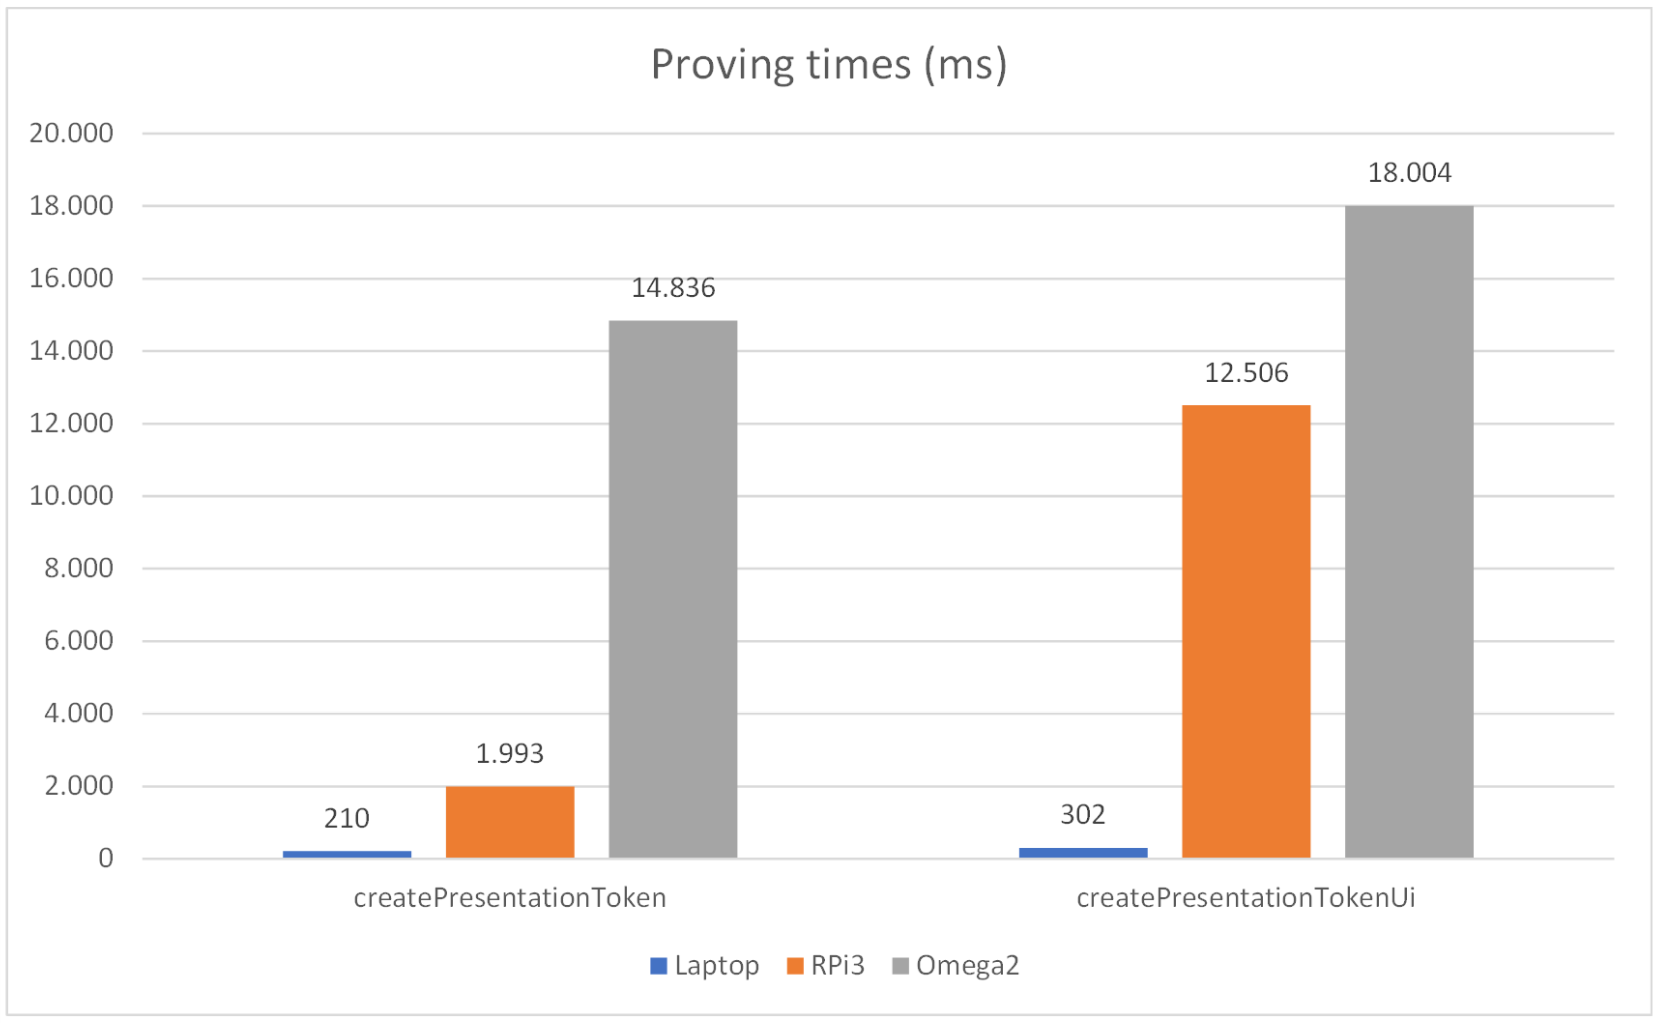
\includegraphics[width=\linewidth]{gfx/graphics/proving}
%	\caption{Proving times (milliseconds). Comparison graph}
%	\label{fig:proving:graph2}
%\end{figure}

Unlike the previous steps, the Presentation or Proving is done more than once, being the key feature of ZKP protocols. The laptop performs a prove in less than one second, the RPi3 needs $15$ seconds, but our P2ABCE IoT deployment needs $15$ seconds for the first step, and $18$s for the second step, $33$ seconds total to generate a Presentation Token.




\hfil

\paragraph{Memory usage on the Omega2}\hfil

Using the tool \textit{time -v} we can get a lot of useful information about a program, once it finishes. In our case, the binary with BIOSC and the smart card logic starts as an empty smart card, goes through the described process, and then we can stop it, as the User Service won't use it anymore.

After another round of tests, now using \textit{time -v}, the field named \textit{Maximum resident set size (kbytes)} shows the \textbf{maximum} size of RAM used by the process since its launch. In our case, this involves the use of static memory for the \textit{global variables} of the smart card logic, and the dynamic memory used by the third party libraries, like GMPlib, OpenSSL and cJSON.

GMP and OpenSSL always allocate the data in their own ADT, what involves copying the arrays of bytes representing the big modular integers from the cryptographic operations. cJSON, used in the serialization of the smart card for storage, and debug being human readable, stores a copy of every saved variable in the JSON tree structure, then creates a string (array of char) with the JSON, that the user can write to a file.

Understanding the many bad uses of memory done in this PoC is important for future improvements and ports. A custom modular library using the same array of bytes that the smart card logic, a binary serialization, and many improvements, are our future work.

With all that said, the mean of the maximum memory usage measured is $6569.6$ kbytes. Compared to the $64$MB of RAM available in the Omega2, our PoC could be executed in more constrained devices, given the system is compatible.




\subsection{Validation conclusions}

Below \autoref{totaltime} sums up the time in seconds used in each step of the test for the Omega2 and Raspberry Pi 3 setup.

The first step, \textit{System Setup} is done only once when the system is being deployed, and the \textit{IoT Smart Card Setup} only once per device.

Because a device can have more than one credential, the Issuance step is significant when we issue multiple credentials over the device's lifetime. We recall that our tests used a credential with five attributes and key sizes of 1024 bits.

Finally, the Proving step is expected to be the most performed calculation by the IoT device. The fact that it lasts over half a minute implies that we should not use this PoC for \textit{real-time} applications yet, usually used in critical secure systems. Nevertheless, for many other IoT applications, the fact this operation can be performed multiple times per hour, presents an useful tool for privacy, e.g. the thermostat system mentioned in the smart building, which can pool data from the sensors every few minutes.


\begin{table}[!ht]
	\begin{center}
		\begin{tabular}{|r|r|r|r|}
			\hline
			System & IoT Smart  & Issue  & Prove Presen-\\
			Setup & Card Setup & credential & tation Policy\\ \hline
			3.77 s & 19.19 s & 36.48 s & 32.84 s \\ \hline
		\end{tabular}
	\end{center}
	\caption{Total time spent for each step in the Omega2+RPi3 setup.}
	\label{totaltime}
\end{table}











%************************************************
\section{Conclusions and Future Work}\label{ch:conclusions}
%************************************************

To finish this document, we sum up some conclusions from the work done, and results 
obtained. We will also enumerate some future lines of research.

\subsection{Conclusions}


In the memory of this project we try to show the work done from the beginning, but we only showed our right decisions, and the information that is significant for the final result. The truth is that, aside from the information included in this paper, we have worked with other systems that ended up discarded. This isn't a negative aspect, because if we didn't, for example, study the Contiki OS, Cooja simulator and the hardware used, we could not be sure the development of the first PoC for that system would be impossible in the time given.


With regard to the work presented, the flexibility of the computation offloading technique, identifying the key operations that can be delegated, and those ones that can't, has allowed us to define a general solution for the vast world of the Internet of Things. The IoT devices can operate as individual actors in the P2ABCE ecosystem, and when in need of performing computation offloading, the delegation server can also be a device considered into the IoT class.


% Resultados son válidos: feseability, problema de tiempo en sistemas de tiempo real
% Se han conseguido objetivos planteados
% Experiencia: qué era más tedioso, dificultades durante diseño y desarrollo
% Primera aproximación de este tipo ~~: más bien somos el future work de...
% Aplicación de procedimientos aprendidos/aplicados durante el TFG/carrera
% ^ Novelty


During the development, we had to investigate a lot of concepts related to IoT, smart cards, and even the insides of P2ABCE's code, to fix many existing bugs in the original project and minimize the amount of changes it had to undergo, in order to work with the IoT devices. In the implementation chapter we give guidelines to port MULTOS applications, considering the particularities we encountered, that's why we can't consider it an \textit{instruction manual to port MULTOS apps}, but an interesting reading on how to confront a similar project. For example, if we wanted the Idemix implementation from \cite{vullers2013efficient}, previous to P2ABCE, in a IoT device, we could apply almost the same steps, obtaining a core functionality of Idemix for constrained devices in C.

Our PoC implementation demonstrates that this project is actually feasible, not by performing a simulation of an IoT device, like in \cite{vanet}. However, the use of third party libraries and no hardware acceleration support, makes the PoC too slow for certain cases, e.g., a Real-Time system requires almost immediate operations, like a car warning that another one is approaching too fast.
There is a long path of research before we can see this design in production, as many decisions depend on the specific deployment in consideration.


%Recalling the objectives listed in \autoref{objectives:section}, we think we accomplish them, except the implementation of a PoC in the most constrained device possible, where we used LEDE to ease our development, and the last objective, where we could have given a use to the PoC, and we leave as part of the future work. In spite of this negative auto-critic, we have to acknowledge that this is the first privacy-preserving ABC implementation for IoT, designed for extensibility, interoperability and maintenance.

Finally, we are very thankful to IBM's grant for the \textit{Privacy Preserving Identity Management applied to IoT} project, which allowed us to get this far. 


\subsection{Future work}


Due to the nature of the project, there exist many options to continue researching in this area.

In the implementation side, we would continue with a second PoC which aimed for more constrained systems, maybe starting with Arduino, or another line of development would be to implement more P2ABCE functionality inside the IoT device. It would be interesting to compare the execution of the current pure software PoC to that with cryptographic hardware support, e.g. using Atmel's chips for SHA, AES and secure memory.

On the design aspect, now that an IoT device can perform P2ABCE operations, we should integrate it in a bigger project, like inside the IdM\footnote{Identity Management - KeyRock \url{https://catalogue.fiware.org/enablers/identity-management-keyrock}} system of FIWARE\footnote{\url{https://www.fiware.org/}}, to issue Idemix credentials to both users and IoT devices. And once the identification is achieved in a privacy-preserving fashion, more applications should be researched, like how the IoT device could benefit from the ZKP cryptography to prove information not issued in its credential, by expanding the P2ABCE presentation policies.

\begin{figure}[bth]
	\begin{center}
		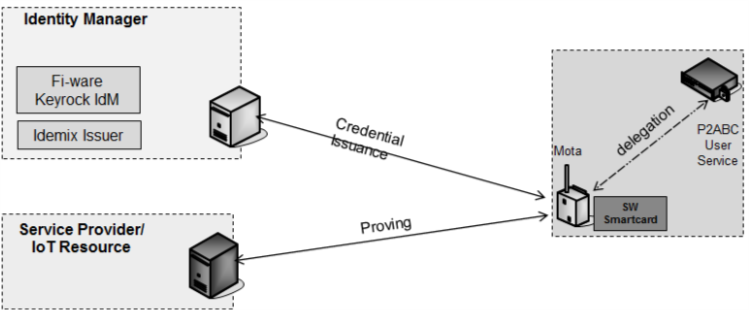
\includegraphics[width=\linewidth]{gfx/fiware}
		\caption{IoT+Idemix Fi-Ware integration.}
	\end{center}
	\label{fig:fiware}
\end{figure}



% trigger a \newpage just before the given reference
% number - used to balance the columns on the last page
% adjust value as needed - may need to be readjusted if
% the document is modified later
%\IEEEtriggeratref{8}
% The "triggered" command can be changed if desired:
%\IEEEtriggercmd{\enlargethispage{-5in}}

% references section

% can use a bibliography generated by BibTeX as a .bbl file
% BibTeX documentation can be easily obtained at:
% http://mirror.ctan.org/biblio/bibtex/contrib/doc/
% The IEEEtran BibTeX style support page is at:
% http://www.michaelshell.org/tex/ieeetran/bibtex/
%\bibliographystyle{IEEEtran}
% argument is your BibTeX string definitions and bibliography database(s)
%\bibliography{IEEEabrv,../bib/paper}
%
% <OR> manually copy in the resultant .bbl file
% set second argument of \begin to the number of references
% (used to reserve space for the reference number labels box)
\bibliography{Bibliography}
\bibliographystyle{plain}


% biography section
% 
% If you have an EPS/PDF photo (graphicx package needed) extra braces are
% needed around the contents of the optional argument to biography to prevent
% the LaTeX parser from getting confused when it sees the complicated
% \includegraphics command within an optional argument. (You could create
% your own custom macro containing the \includegraphics command to make things
% simpler here.)
%\begin{IEEEbiography}[{\includegraphics[width=1in,height=1.25in,clip,keepaspectratio]{mshell}}]{Michael Shell}
% or if you just want to reserve a space for a photo:

%\begin{IEEEbiography}{Michael Shell}
%Biography text here.
%\end{IEEEbiography}

% if you will not have a photo at all:
%\begin{IEEEbiographynophoto}{John Doe}
%Biography text here.
%\end{IEEEbiographynophoto}

% insert where needed to balance the two columns on the last page with
% biographies
%\newpage

%\begin{IEEEbiographynophoto}{Jane Doe}
%Biography text here.
%\end{IEEEbiographynophoto}

% You can push biographies down or up by placing
% a \vfill before or after them. The appropriate
% use of \vfill depends on what kind of text is
% on the last page and whether or not the columns
% are being equalized.

%\vfill

% Can be used to pull up biographies so that the bottom of the last one
% is flush with the other column.
%\enlargethispage{-5in}



% that's all folks
\end{document}


